%!TEX root = ../../dissertation.tex
%%%%%%%%%%%%%%%%%%%%%%%%%%%%%%%%%%%%%%%%%%%%%%%%%%%%%%%%%%%%%%%%%%%%%%%%%%%%%%%%
%\section{Background}
%\label{c4:background}
\section{Mobile Network Architecture}
\label{c4:3gpparchitecture}

This section starts with a primer on cellular data network basics, and then moves on to describe relevant details of \gls{gtp}, the tunneling protocol under investigation.

Today's dominating commercial mobile network system, which includes \gls{GSM}, \gls{UMTS}, and up to \gls{LTE}, is designed and specified by the \gls{3GPP}. This group is an umbrella organization for several standardization bodies, including the European \gls{ETSI} and their individual members --- in this case mostly telecommunication companies. Unlike the \gls{IETF}, the Internet's de facto standards body, natural persons cannot participate in the \gls{3GPP} on their own but only through the organizational members.

Specifications are not released individually but are instead grouped together into larger releases once every or every other year. \gls{GSM} was first specified in the Phase 1 release in 1992 with \gls{GPRS} added in Release 97 (1998). \gls{UMTS} followed with Release 99 (2000), but most 3G networks operate at least with Release 5 (2002), 6 (2004), or 7 (2007) as they introduced \gls{HSDPA}, \gls{HSUPA}, and \gls{HSPA+} likewise. \gls{LTE} first found its way into the specifications in 2008 with Release 8 with Release 12 currently being worked on. This background section mostly describes the \gls{UMTS} based \gls{TS} with some comparisons being made to the older \gls{GPRS} and the latest \gls{LTE} specification versions where available.

\begin{figure}[htbp]
	\centering
 	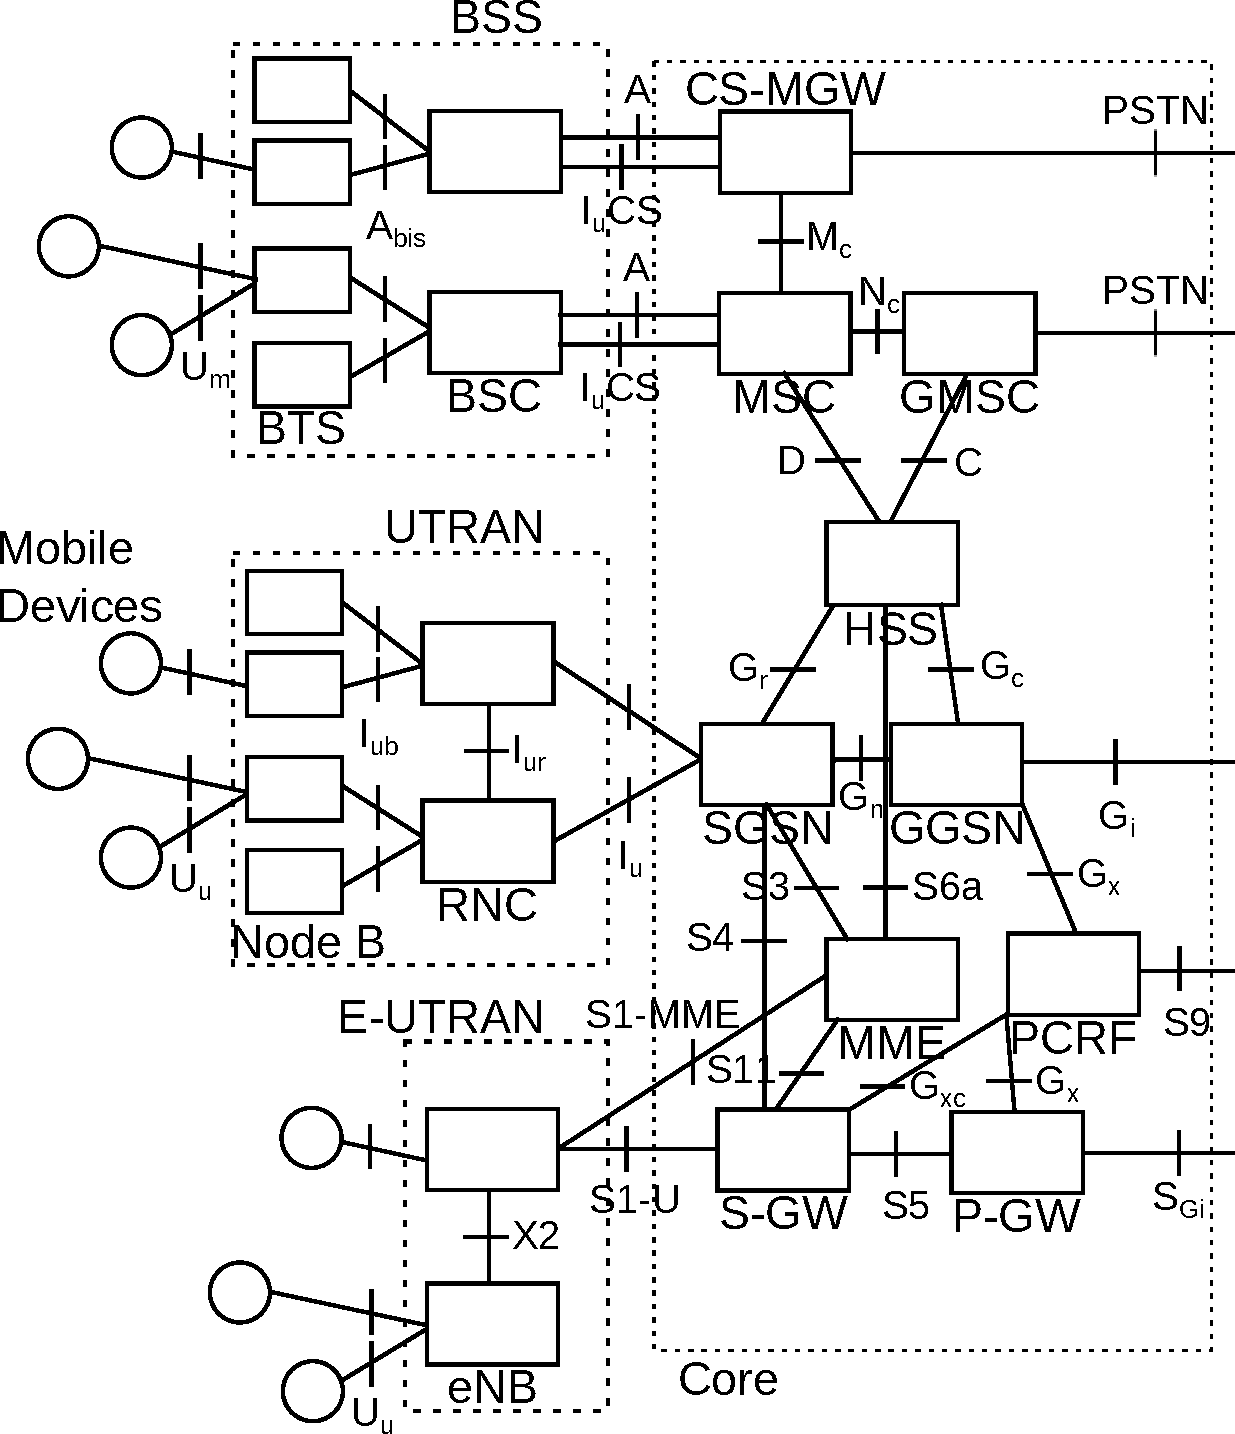
\includegraphics[width=1.0\textwidth]{images/3gpp-physical-arch.pdf}
 	\caption{Combined CS/PS GSM/UMTS/LTE architecture overview.}
 	\label{c4:fig:psdomain}
\end{figure}

Today's most common version of the mobile network architecture is depicted in Figure~\ref{c4:fig:psdomain} and based on 3GPP TS 23.002~\cite{3gpp.23.002}, with some minor nodes and network paths omitted\footnote{For a complete reference of all the acronyms and addressing schemes used in 3GPP specs please refer to TS 21.905~\cite{3gpp.21.905}. and TS 23.003~\cite{3gpp.23.003}}. The displayed architecture combines all three access technologies as well as the \gls{CS} and the \gls{PS} domain of the core. Concerning the \gls{PS} domain, one has to further distinguish between links and nodes used solely for control plane tasks as well as links and nodes that are in path of the actual user IP traffic. For \gls{UMTS} and \gls{GPRS}\footnote{\gls{GPRS} provides \gls{PS} data services for \gls{GSM} radio access. The same core infrastructure is also used in the \gls{UMTS} \gls{PS} domain.} the \gls{SGSN} and the \gls{GGSN} are the core in-band elements. 

One thing to keep in mind is the strict separation between user plane and control plane tasks in the \gls{3GPP} architecture. Usually completely separate protocol stacks are used and signaling is mostly very explicit and out of band. This is contrary to the typical approach of the Internet's stack, especially its upper layers, where most state is implicitly inferred and only some signaled in-band. The following paragraphs give a short description of nodes, general and \gls{PS} tasks handled by them, and used protocols and stacks in the two major network domains inside the infrastructure domain~\cite{3gpp.23.101} for both the user and the control plane. The description will be mostly focused on the \gls{UMTS} parts of the architecture


%%
\subsection{\texorpdfstring{\acrshort{3GPP}}{3GPP} Radio Network}

The architecture has three completely distinct radio networks, one for each access technology: \gls{GSM}'s \gls{BSS} (or more complete: \gls{GERAN}), \gls{UTRAN} for \gls{UMTS}, and \gls{E-UTRAN} in \gls{LTE}.

Essential to the radio network is a base station, a radio transceiver providing the physical connection to the user's mobile device\footnote{Mobile devices are called \gls{MS} in \gls{GSM} networks and \gls{UE} in 3G and later.} 3G's base station is called Node B. The used radio spectrum is divided into a number of channels, with various shared channels responsible for management and control plane signaling and one or more dedicated channel for each active mobile device~\cite{3gpp.25.201,3gpp.25.301}. Layer 2 consists of several protocols managing and multiplexing transmissions on the link. These are \gls{MAC}~\cite{3gpp.25.321} and \gls{RLC}~\cite{3gpp.25.322} with an additional user plane broadcast service provided by \gls{BMC}~\cite{3gpp.25.324}. On Layer 3, the actual radio control plane signaling protocol \gls{RRC}~\cite{3gpp.25.331} resides, managing the device's state and the radio connection. Some of the signaling procedures are detailed in \cite{3gpp.25.931}. Additionally, \gls{PDCP}~\cite{3gpp.25.323} provides the connection to the  usual Internet TCP/IP userplane stack atop. Thus, all user traffic is encapsulated into so called \textit{radio bearers}, which tunnels traffic from the mobile device directly into the core network.

Each base station acts as an independent radio cell. Mobile devices can be handed over between cells without higher layers being able to notice this.\footnote{However, there are still many ways to detect a handover in the upper layers of a mobile device.} The handover process is fully controlled and conducted by the network by a node that shares the old and new path to the device. For \gls{UMTS}, in most cases this can be handled by the \gls{RNC} while the core \gls{SGSN} is responsible for handovers between regions.

	
In \gls{UMTS} multiple Node B are concentrated into one \gls{RNC}. Most of the functions of a \gls{RNC}, including mobility management, are defined by the \gls{RANAP} control plane protocol \cite{3gpp.25.413}. \gls{RANAP} is used in the Iu interface between the \gls{RNC} and the core network, i.e. the \gls{SGSN}. All non-radio links of the network are today \gls{IP}-based, but in the past all interfaces have also been explicitly defined for \gls{ATM} with some differences to the \gls{IP}-based stack. The connection of the decentralized parts of the radio network to either the core network itself or a \gls{RNC} is called \textit{backhaul}. This term usually subsumes the bulk transport of data over dedicated links to a central location. Often, optical fiber or microwave transmission links are used.



%%
\subsection{\texorpdfstring{\acrshort{3GPP}}{3GPP} Core Network}

The \gls{PS} domain of a mobile core network manages most of the aspects of the connected devices and acts as the bridge to the Internet. It consists of nodes that are directly in the path of the user plane traffic as well as additional nodes, that only exist in the control plane.

\gls{GPRS} and \gls{UMTS} use the exact same \gls{PS} core network architecture, only \gls{LTE} introduced a new core network concept, the \gls{EPC}. If the same core is used for both (or all three) access technologies, nodes for all architecture versions have to be present with the exception of some control plane nodes, that \gls{EPC} replaces with its counterparts that provide legacy interfaces.

The two central elements in the userplane's path are the \gls{SGSN} and the \gls{GGSN}~\cite{3gpp.22.060,3gpp.23.060}. The \gls{SGSN} is the endpoint of the \gls{RAB}, tunneling user traffic from the \gls{UE} to the core, and an endpoint for the \gls{gtp} based core tunnel, further transporting userplane traffic to the \gls{GGSN}. \gls{gtp} will be described in detail in Section~\ref{c4:sec:gtp}. The \gls{GGSN}'s control plane tasks include mobility and connection management via \gls{RANAP} to the gls{RNC}. The necessary information is cached and retrieved from the \gls{HLR}  using \gls{MAP}~\cite{3gpp.29.002}. The \gls{HLR} or, respectively, the \gls{HSS} in an \gls{EPC}, acts as the central storage of all the operator's subscriber information.

The \gls{GGSN} represents the gateway to the public Internet and therefore typically is the only node in the network, that has a publicly routable \gls{IP} address. It filters incoming traffic into the corresponding \gls{gtp} tunnel and routes packets to the correct \gls{SGSN}. State about any active tunnel and device has to be kept locally and is initially retrieved from the \gls{SGSN}.

In \gls{EPC} user traffic in the core is handled by the \gls{SGW} and \gls{PGW}, having similar functions as their \gls{GPRS} counterparts \gls{SGSN} and \gls{GGSN}. Depending on the specific implemented infrastructure these two nodes can also be combined into one, eliminating the S5 interface and the \gls{gtp} signaling between them. Much of the control plane tasks of the \gls{SGSN} have now been offloaded to a new node, the \gls{MME}, which maintains its own logical connection to the radio network using the \gls{S1AP} signaling protocol~\cite{3gpp.36.413}. Instead of \gls{MAP} to retrieve user data from the central storage, Diameter~\cite{rfc6733} is now used to communicate with the \gls{HSS}. Of note is also a further addition to the \gls{EPS}: the \gls{PCRF} in conjunction with the \gls{PCEF} integrated into the \gls{PGW}. They act as a \gls{DPI} entity, inspecting all userplane traffic and enable arbitrary filtering of traffic and traffic-based billing~\cite{3gpp.23.203}. 

	

%%
\subsection{Core Network Concepts and Protocol Details}


All core network signaling procedures and state machines are specified in TS 24.008~\cite{3gpp.24.008}

simple example procedure:
	\gls{PDP} context activation procedure in \gls{UMTS}
	invokes additional \gls{CAMEL} procedures defined in \cite{3gpp.23.078}

	\begin{figure}[htb]
		\centering
		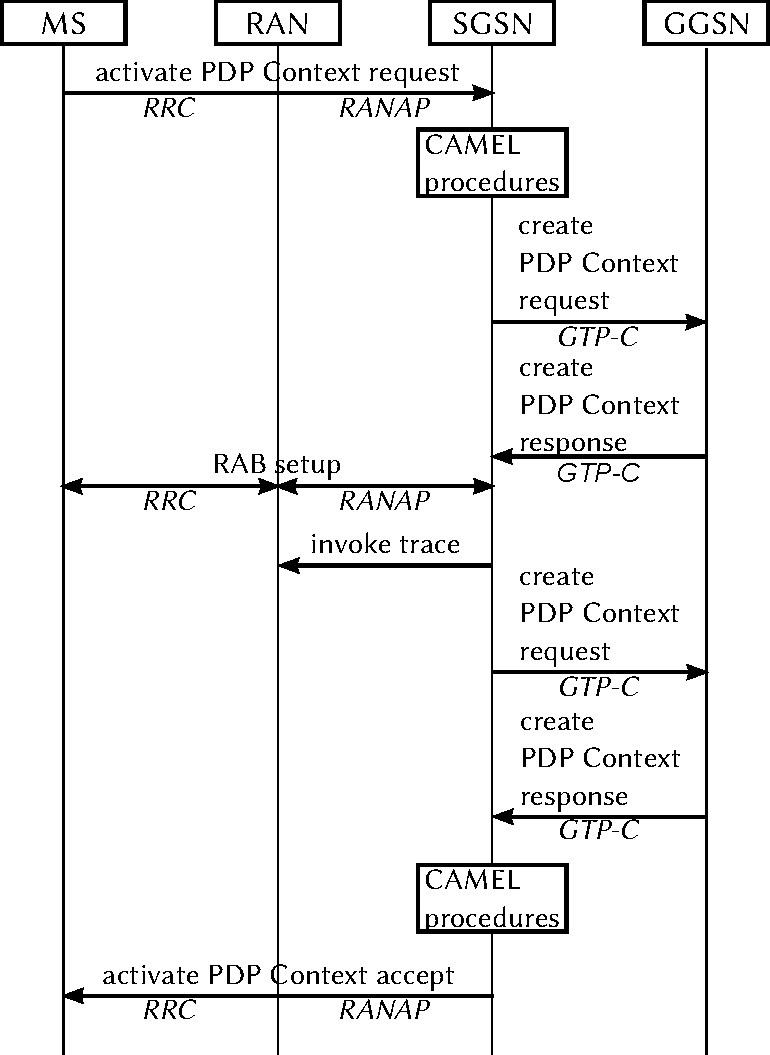
\includegraphics[width=0.7\textwidth]{images/pdp-context-activation-procedure.pdf}
		\caption{PDP Context Activation procedure signaling interaction diagram for \gls{UMTS}, including involved signaling protocols.}
		\label{c4:fig:pdpcontextactivationinteraction}
	\end{figure}

	29.060 \cite{3gpp.29.060} GTPv1 description; GPRS/UMTS version; Gn (SGSN - GGSN) Gp interfaces
	29.281 \cite{3gpp.29.281} GTPv1-U user traffic tunnel description
	29.274 \cite{3gpp.29.274} GTPv2-C protocols and procedures (LTE only) on S5 (S-GW - P-GW) and S8 (P-GW - P-GW) interfaces

%%
\subsubsection{Mobile Network Control Plane}

separation between control and user plane: tunneling concept
state machines
protocols
procedures -> location of control inside the network vs at the edge
comparison of explicit (3G) control networks vs implicit (IP)
resulting complexity
...



%%
\subsubsection{State Keeping: \texorpdfstring{\acrshort{PDP}}{PDP} Context Concept}
explain data structure/state



%%
\subsubsection{\texorpdfstring{\acrshort{gtp}}{GTP} and \texorpdfstring{\acrshort{gtp}}{GTP}-based Core Network Signaling}
\label{c4:sec:gtp}





\begin{figure}[htb]
	\centering
	\includegraphics[width=1.0\textwidth]{images/3g-userplane.pdf}
	\caption{User plane protocol stack in an UMTS network.}
	\label{c4:fig:3gpp-umtsuserplane}
\end{figure}

% \begin{figure}[htb]
% 	\centering
% 	\includegraphics[width=1.2\textwidth]{images/LTE-userplane.pdf}
% 	\caption{User plane protocol stack in an LTE/EPC network.}
% 	\label{c4:fig:3gpp-lteuserplane}
% \end{figure}





%%
\paragraph{Tunneling Concept and Bearers}

LTE: mention also \gls{PMIP} as \gls{gtp} alternative, and the option to have a combined \gls{SGW} \gls{PGW}


One UE Can have a maximum of 3 \gls{PDN} connections and 11 bearers (one default per \gls{APN} and additional dedicated).


\begin{figure}[htb]
	\centering
	\includegraphics[width=1.0\textwidth]{images/bearers.pdf}
	\caption{3GPP bearer model.}
	\label{c4:fig:3gpp-bearers}
\end{figure}


% \begin{figure}[htb]
% 	\centering
% 	\includegraphics[width=1.2\textwidth]{images/ECM-states.pdf}
% 	\caption{\gls{ECM} state machine.}
% 	\label{c4:fig:3gpp-ecmstates}
% \end{figure}

\begin{itemize}
\item 	Every bearer has a predefined QoS level between UE and P-GW.
		==> Level of Granularity for QoS control.
\item	Initial bearer QoS level assigned by network based on subscription data.
\item	Guaranteed Bit Rate (GBR) bearers: dedicated network resources permanently allocated at est/mod. Otherwise Non-GBR.
\item	The Traffic Flow Template (TFT) belonging to a bearer is a set of packet filters that assign traffic flows to the bearer.
\item	UL-TFT at UE, DL-TFT at \gls{PCEF} (P-GW).
\item 	default bearer: always-on IP connectivity for the UE to a PDN
\item	dedicated bearer:   
			\begin{itemize}
				\item any additional bearer for the same PDN
				\item \gls{TFT} associated with every ded. bearer
				\item establishment/modification decision only by \gls{EPC}
				\item QoS level assignment only by \gls{EPC}
			\end{itemize}

\item	default bearer may be used as {m,c}atch-all traffic bearer for everything that does not match any filter
\item	Every bearer associated with QCI and ARP.

QoS class identifier (QCI): standardized scalar as reference for node-specific QoS parameters
Allocation and Retention Policy (ARP): priority level preemption capability, preemption vulnerability.

\item	All simultaneously active bearers by one UE are provided are provided by the same P-GW.
\end{itemize}



%%
\subsubsection{\texorpdfstring{\acrshort{GPRS}}{GPRS} Fundamentals}

The packet switched domain of an \gls{UMTS} network is an evolution of \gls{GPRS} and thus closely related to it. First defined by the \gls{3GPP} in Release 99, it focuses its improvements over \gls{GSM} mostly on the radio aspects, while keeping the core network \gls{GPRS} architecture intact at large. \gls{3GPP} \gls{TS} 23.060 \cite{3gpp.23.060} defines the basic aspects involving \gls{GPRS} protocols and its system architecture. \gls{TS} 29.060 \cite{3gpp.29.060} describes the specifics of \gls{gtp} flowing across the Gn and Gp interfaces which forms the foundation for our work.



As shown in Figure \ref{c4:fig:psdomain}, user traffic originating at any \gls{MS} connected to the radio network flows through a Node B (also called base station), which provides radio connectivity. Multiple Node B are aggregated into a \gls{RNC}. The base stations and \glspl{RNC} form the \gls{UTRAN}, which is typically connected by back-haul fiber links to the core network part formed by the \gls{SGSN} and the \gls{GGSN}.

One role of the \gls{SGSN} is to serve as mobility anchor for mobile devices. It is also the endpoint for \gls{RRC}-based signaling and the \gls{RAB}, the radio counterpart to the core network user traffic tunnel. The \gls{GGSN} provides the gateway to the public Internet. The Gn interface connects those two nodes, using the \gls{gtp} protocol to encapsulate user as well as control plane traffic as seen in the protocol stack in Figure \ref{c4:fig:signallingstack}. \gls{gtp} is further separated into GTP-C, facilitating control message exchange, and GTP-U for transporting user traffic through tunnels in the core.

\begin{figure}[htb]
	\centering
	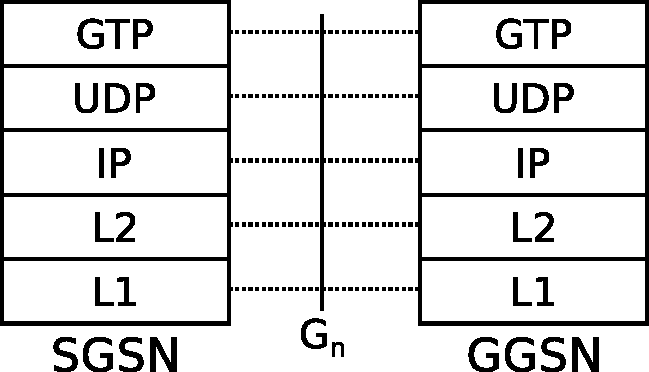
\includegraphics[width=0.6\columnwidth]{images/signalling-stack.pdf}
	\caption{Typical signaling protocol stack at the Gn interface between \gls{SGSN} and \gls{GGSN}.}
	\label{c4:fig:signallingstack}
\end{figure}


Before diving into specifics of \gls{gtp} messaging, we give a short overview on the packet switched domain of an \gls{UMTS} network. This domain is closely related to the \gls{GPRS} part introduced for \acrshort{GSM}. \gls{UMTS}, first defined by the \gls{3GPP} in Release 99, focuses its improvements over \gls{GSM} mostly on the radio aspects, while keeping the core network \gls{GPRS} architecture intact at large. \gls{3GPP} \gls{TS} 23.060 \cite{3gpp.23.060} defines the basic aspects involving \gls{GPRS} protocols and its system architecture. \gls{TS} 29.060 \cite{3gpp.29.060} describes the specifics of \gls{gtp} flowing across the Gn and Gp interfaces which forms the basis for our work.

As shown in Figure \ref{c4:fig:psdomain}, user traffic originating at any \gls{MS} connected to the radio network flows through one of the Node Bs, providing radio connectivity. Multiple Node Bs are aggregated by a \gls{RNC}. Node Bs and \glspl{RNC} form the \gls{UTRAN}, which is typically connected by back-haul fiber links to the core network part formed by the \gls{SGSN} and the \gls{GGSN}.

One role of the \gls{SGSN} is as the mobility anchor for mobile devices, and it is the endpoint for \gls{RRC}-based signaling and the \gls{RAB}. The \gls{GGSN} provides the gateway to the public Internet. The Gn interface connects those two nodes, using the \gls{gtp} protocol to exchange user as well as control plane traffic as seen in the protocol stack in Figure \ref{c4:fig:signallingstack}. \gls{gtp} is further separated into GTP-C, facilitating control message exchange, and GTP-U for transporting user traffic through tunnels.







% \subsubsection{Information Element Concept}
% Discuss the concept
% list all involved IEs their sizes and thus the imposed overhead
% "The IMSI IE together with the NSAPI IE uniquely identifies the PDP context to be created"

\begin{table}[htb]
	\caption{GTP header format (TODO: which one exactly. This looks like v2-U but should actually better be v1!)}
	\label{c4:tbl:gtpheader}
	\begin{tabu}{c|c|c|c|c|c|c|c|c|}
	\multicolumn{1}{c}{} & \multicolumn{8}{c}{\textbf{Bits}} \\
	\cline{2-9} \textbf{Octets} & 8 & 7 & 6 & 5 & 4 & 3 & 2 & 1 \\ 
	\cline{2-9} 1 & \multicolumn{3}{c|}{Version}  & P & T & Spare & Spare & Spare \\ 
	\cline{2-9} 2 & \multicolumn{8}{c|}{Message Type}  \\ 
	\cline{2-9} 3 & \multicolumn{8}{c|}{Message Length (1st Octet)}  \\ 
	\cline{2-9} 4 & \multicolumn{8}{c|}{Message Length (2nd Octet)}  \\ 
	\cline{2-9} m to & \multicolumn{8}{c|}{\multirow{2}{10cm}{If T flag is set to 1, then TEID shall be placed into octets 5-8. Otherwise, TEID field is not present at all.}} \\ 
	 k(m+3) & \multicolumn{8}{c|}{} \\ 
	\cline{2-9} n to (n+2) & \multicolumn{8}{c|}{Sequence Number} \\ 
	\cline{2-9} (n+3) & \multicolumn{8}{c|}{Spare} \\ 
	\cline{2-9} 
	\end{tabu} 
\end{table}


\begin{table}[htb]
	\caption{12 Byte GTPv2-C header format.}
	\label{c4:tbl:gtpv2cheader}
	\begin{tabu}{c|c|c|c|c|c|c|c|c|}
	\multicolumn{1}{c}{} & \multicolumn{8}{c}{\textbf{Bits}} \\
	\cline{2-9} \textbf{Octets} & 8 & 7 & 6 & 5 & 4 & 3 & 2 & 1 \\ 
	\cline{2-9} 1 & \multicolumn{3}{c|}{Version}  & P & T=1 & Spare & Spare & Spare \\ 
	\cline{2-9} 2 & \multicolumn{8}{c|}{Message Type}  \\ 
	\cline{2-9} 3 & \multicolumn{8}{c|}{Message Length (1st Octet)}  \\ 
	\cline{2-9} 4 & \multicolumn{8}{c|}{Message Length (2nd Octet)}  \\ 
	\cline{2-9} 5 & \multicolumn{8}{c|}{Tunnel Endpoint Identifier (1st Octet)} \\ 
	\cline{2-9} 6 & \multicolumn{8}{c|}{Tunnel Endpoint Identifier (2nd Octet)} \\ 
	\cline{2-9} 7 & \multicolumn{8}{c|}{Tunnel Endpoint Identifier (3rd Octet)} \\ 
	\cline{2-9} 8 & \multicolumn{8}{c|}{Tunnel Endpoint Identifier (4th Octet)} \\ 
	\cline{2-9} 9 & \multicolumn{8}{c|}{Sequence Number (1st Octet)} \\
	\cline{2-9} 10 & \multicolumn{8}{c|}{Sequence Number (2nd Octet)} \\
	\cline{2-9} 11 & \multicolumn{8}{c|}{Sequence Number (3rd Octet)} \\
	\cline{2-9} 12 & \multicolumn{8}{c|}{Spare} \\
	\cline{2-9}
	\end{tabu} 
\end{table}

Table~\ref{c4:tbl:gtpheader} lists the standard GTPv1 header format used in any GPRS and 3G network.

Table~\ref{c4:tbl:gtpv2cheader} lists the default header format for a GTPv2-C message used in \gls{LTE} networks.


request/response messaging
response types:
Possible context response types and which request types they answer:
\begin{itemize}
\item 192: ``non-existent'' UPDATE \& DELETE ONLY
\item 193: ``invalid message format'' UPDATE \& DELETE ONLY
\item 199: ``no resources available'' CREATE ONLY anywhere in the network to allocate context
\item 200: ``service not supported'' UPDATE ONLY
\item 201: ``mandatory IE incorrect''
\item 202: ``mandatory IE missing''
\item 204: ``system failure'' CREATE \& UPDATE ONLY
\item 209: ``user authentication failed'' CREATE ONLY rejected for various reasons
\end{itemize}

\gls{IE} calculation basis
\begin{table}[htb]
\caption{Information Elements in a Create PDP Context Request (as peer TS 29.060, Section 7.3.1)}
\label{tab:createrequestelements}
\begin{tabular}{|p{4cm}|p{2cm}|p{2cm}|p{4cm}|p{2cm}|p{2cm}|} \hline
\textbf{Information Element} & \textbf{Presence Requirement} & \textbf{Typical Size} & \textbf{Information Element} & \textbf{Presence Requirement} & \textbf{Typical Size} \\ \hline
IMSI & Conditional & 9 & TFT & Conditional & min. 4\\ \hline
Routing Area Identity & Optional & 7 & Trigger Id & Optional & min. 4 \\ \hline
Recovery & Optional & 2 & OMC Identity & Optional & min. 4 \\ \hline
Selection mode	& Conditional & 2 & Common Flags & Optional & 4\\ \hline
Tunnel Endpoint Identifier Data I & Mandatory & 5 & APN Restriction & Optional & 4\\ \hline
Tunnel Endpoint Identifier Control Plane & Conditional & 5 & RAT Type & Optional & 4\\ \hline
\gls{NSAPI} & Mandatory & 2 & User Location Information & Optional & 11\\ \hline
Linked NSAPI & Conditional & 2 & MS Time Zone & Optional & 5\\ \hline
Charging Characteristics & Conditional & 3 & IMEI(SV) & Conditional & 11\\ \hline
Trace Reference & Optional & 3 & CAMEL Charging Information Container & Optional & min. 4\\ \hline
Trace Type & Optional & 3 & Additional Trace Info & Optional & 12\\ \hline
End User Address & Conditional & 9 (for IPv4) & Correlation-ID & Optional & 4\\ \hline
Access Point Name & Conditional & 3 + Name & Evolved Allocation Retention Priority I & Optional & 4\\ \hline
Protocol Configuration Options & Optional & min. 3 & Extended Common Flags & Optional & min. 4\\ \hline
SGSN Address for signaling & Mandatory  & 9 (for IPv4) & User CSG Information & Optional & 11 \\ \hline
SGSN Address for user traffic & Mandatory & 9 (for IPv4) & APN-ABMR & Optional  & 11 \\ \hline
MSISDN & Conditional & 3 + MSISDN & Max MBR/APN-ABMR & Optional & min. 11 \\ \hline
QoS Profile & Mandatory & min. 5 & Private Extension & Optional & min 6\\ \hline
Signaling Priority Indication & Optional & min. 4 & & & \\ \hline
\end{tabular}
\end{table}

GTP Header: 12 Byte
IE header and footer: 2 Byte
Maximum minimum data size including all \glspl{IE}: 221 Byte + 12 Byte Header + 2*37 Extension Header = 307 Byte
Minium size of mesage with just mandatory \glspl{IE}: 12 + 30 + 2*5 = 52 Byte

307 Bytes:
calculation from our dataset
Total maximum signaling traffic with this calculation: 117.15GB
Ratio: 0.10\%
52 Bytes:
Total maximum signaling traffic with this calculation: 19.84GB
Ratio: 0.02\%
Total traffic: 122758578593993

Tunnels state is held in the \gls{SGSN} and \gls{GGSN} as \gls{PDP} Context data structures. These contain various information, such as the device IP address, \gls{IMSI}, and a tunnel identifier. The concept is used to isolate user traffic from core network control plane signaling and to provide certain \gls{QoS} guarantees to the user traffic. Multiple \gls{QoS} profiles per device can also be established by setting up up to ten secondary contexts beyond the primary PDP context. However, \gls{QoS} secondary contexts are very rarely in use today, any user-plane IP traffic is typically transported within the primary ``best effort'' tunnel.

The GTP-C signaling, responsible for the context management interactions, contains procedures for managing data paths, \gls{MS} locations, mobility, and, of course, tunnels. \gls{gtp} messages usually come as request-response pairs. Neither part has fixed size, but is rather constructed from a number of \glspl{IE}, many of which are either optional or variable length through additional optional fields.

The focus of our work will be the three Tunnel Management message pairs involved in the maintenance of PDP Contexts. These are:

\begin{itemize}
\item The \textbf{Create Context Message}, which is part of several larger control procedures that activate the GTP tunnel for a mobile device. These can be initiated from the network as well as the device itself, again depending on the specific implementation of the architecture. When a \gls{GGSN} receives this request from an \gls{SGSN}, it attempts to complete the Context creation. Depending on the outcome, a response is sent back, indicating the success or failure of the operation. Typical failures include failed user authentication, lack of resource, or unrecoverable system failures.

\begin{figure}[htb]
	\centering
	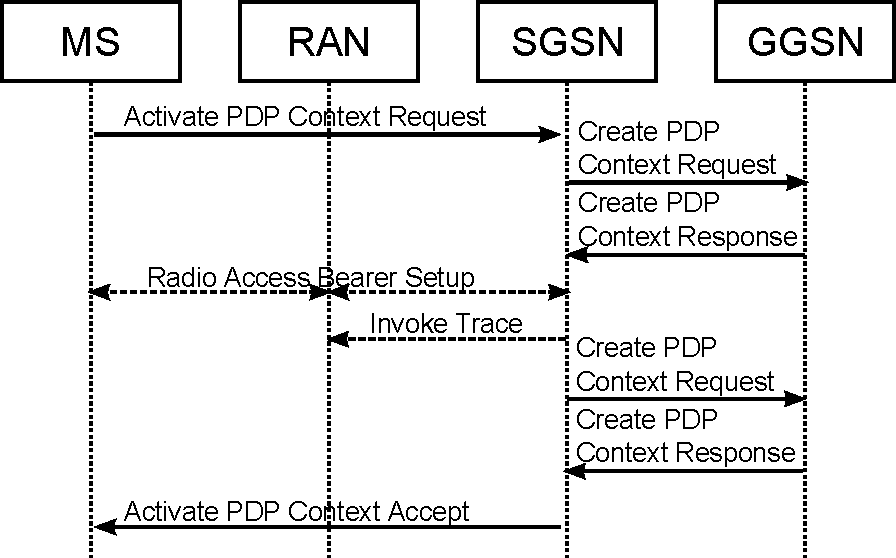
\includegraphics[width=0.8\columnwidth]{images/pdp-context-activation.pdf}
	\caption{PDP Context Activation Procedure in a UMTS network.}
	\label{c4:fig:pdpcontextactivation}
\end{figure}

Figure \ref{c4:fig:pdpcontextactivation} shows the \textit{PDP Context Activation Procedure} as defined in \cite{3gpp.23.060}. Some additional \gls{CAMEL} procedures may be involved in the creation but are not of interest in the context of this paper as they are not required. Tunneling messages are usually triggered by other procedures on different interfaces. In the case depicted here, the procedure is initiated by the mobile device through a \gls{RANAP} protocol \textit{Activate PDP Context Request} typically sent when establishing a mobile data connection.

Generally speaking, any Create Request is part of a \textit{GPRS PDP Context Activation} procedure, which can happen under several circumstances, the aforementioned one being the typical, but also during each \textit{Secondary PDP context Activation} procedure for every tunnel beyond the first. When a \gls{GGSN} receives this request from an \gls{SGSN}, it attempts to complete the Context creation. Depending on the outcome, a response is sent back, indicating the success or failure of the operation. Typical failure codes observed in our measurements were either due to incorrect information supplied by the device (``user authentication failed''), due to malformed messages (e.g. ``invalid message format''), or indicated problems or temporary overload in the network (``no resources available'' and ``system failure'').



\item \textbf{Delete Context Message}; This indicates the immediate release of the Context involved. 
Together with the Create event these mark the beginning and the end of every GTP tunnel, making them good candidates to determine tunnel durations for our load evaluations.

The third type of Tunnel Management messages are the \textit{Delete Context Request} and \textit{Response}, indicating the immediate release of the Context involved. They are part of 

\begin{itemize}
	\item The \textit{GPRS Detach} procedure from the \gls{SGSN} to the \gls{GGSN}, when a device completely deactivates its data services.
	\item The \textit{GPRS PDP Context Deactivation} procedure from the \gls{SGSN} to the \gls{GGSN}, if only one specific tunnel is to be removed.
	\item The \textit{part of PDP Context Deactivation Initiated by GGSN} procedure signaled to the \gls{SGSN}.
\end{itemize}
%can also delete a set of contexts assigned to a single MS


\item \textbf{Update Context Messages}; Several procedures also emit tunnel update messages, when some aspect of the tunnel has changed, e.g. occurring in mobility and load-balancing related procedures but also procedures involving secondary tunnels for a device.
By observing Update Context message one could, for example, capture most forms of mobility happening in the network, and get a good picture of correlations between mobility and tunneling characteristics. 

The possible causes for an \textit{Update Context Request} are as following.

\begin{itemize}
	\item The mobile devices moves between \glspl{SGSN}, causing a \textit{GPRS inter-SGSN Routing Area Update} procedure.
	\item Parameters belonging to the context such as the assigned \gls{QoS} are altered using the the \textit{PDP Context Modification}.
	\item As part of \textit{Context redistribution and load balancing} procedures.
	\item The \gls{MS} switches between \gls{UMTS} and \gls{GPRS} access technologies, causing a \textit{Inter-system intra- \\SGSN Update} procedure. Note that the same tunnel can be used regardless of the radio technology.
	\item As part of a direct \gls{RNC} to \gls{GGSN} GTP-U tunnel activation procedure, thereby circumventing the \gls{SGSN}. Or, finally, 
	\item To activate secondary PDP contexts using the \textit{Secondary PDP Context Activation} as previously described. 
\end{itemize}

By observing Update Context message one could, for example, capture most forms of mobility happening in the network, and get a good picture of correlations between mobility and tunneling characteristics. Additionally, tunnels using \gls{UMTS} and \gls{GPRS} radio technology can be distinguished, which should in theory lead to wholly different pictures, as nowadays GSM/GPRS is either used in older models or feature phones, or in mobile scenarios in rural areas where the larger GSM cells are more prevalent. Both could indicate that the data session will be rather short  due to either clumsy devices or the low throughput rates of \gls{GPRS}.
\end{itemize}

The variable-length nature of these messages makes evaluating the imposed network signaling overhead rather difficult. For example, the Create Context Response consists of up to 36 \glspl{IE}, some of them mandatory, most either conditional or optional. Including the headers of both the packet and the individual elements, the minimum size (counting only the required bytes of variable length elements) is 52 bytes, while the lower bound for the message size with all \glspl{IE} present is 307 bytes.

Taking the maximum size we arrive at a naive estimate of the maximum overhead on user traffic induced by tunnel management signaling in our dataset. The estimated ratio of (tunnel management) signaling traffic to total user plane traffic in our dataset is a minute $0.10\%$. Therefore, the volume of control plane traffic appears to be non-critical in this setup. Thus, we assume that the overload problems mentioned above arise rather in areas affected by signaling except for the pure transport of data, such as the memory profile of the states kept in the gateway nodes, the time required to process the large number of information held in the messages, or the imposed latency through several message round trips during transactions.

%%

Tunnels are defined in the \gls{SGSN} and \gls{GGSN} in \gls{PDP} Context data structures. These hold various information related to a tunnel, such as the device IP address, \gls{IMSI}, and a tunnel identifier. A tunneling concept is used for user traffic to isolate it from core network control plane traffic and to provide certain \gls{QoS} guarantees to the user traffic. To distinguish multiple \gls{QoS} profiles per device, up to ten additional secondary contexts can be established beyond the primary PDP context, all with different \gls{QoS} allocations. However, secondary contexts are rarely in use today, and any user-plane IP traffic is transported within the primary ``best effort'' tunnel.

As already mentioned, GTP-C signaling is used to administer these contexts. Across the Gn path, it contains procedures for managing data paths, \gls{MS} locations, mobility, and, of course, tunnels. We take a specific look at the last one. \gls{gtp} messages usually come as request-response pairs. Neither part has fixed size, but is rather constructed from a number of \glspl{IE} of partially variable length. 

The focus of our work will be the three Tunnel Management message pairs involved in the maintenance of PDP Contexts. These are the \textit{Create, Update,} and \textit{Delete PDP Context Requests} and \textit{Responses}. Each pair, including their causes and possible effects, will be treated in a separate section, with the Create and Delete messages forming the substrate for our investigations presented in this paper.

The variable-length nature of these messages makes evaluating the imposed network signaling load rather difficult. For example, the Create Context Response consists of up to 36 \glspl{IE}, some of them mandatory, most either conditional or optional. Including the headers of both the packet and the individual elements, the minimum size (counting only the required bytes of variable length elements) is 52 bytes, while the minimal maximum size with all \glspl{IE} present is 307 bytes.

Taking this maximum value we arrive at a naive estimate of the maximum overhead on user traffic imposed by tunnel management signaling in our dataset. The ratio of (tunnel management) signaling traffic to total user plane traffic is a minute $0.10\%$. Therefore, the sheer volume of control plane traffic appears to be non-critical in this setup. We assume thus that the overload problems mentioned above arise rather in areas affected by signaling except for the pure transport of data, such as the memory profile of the states kept in the gateway nodes, the time required to process the large number of information held in the messages, or the imposed latency through several message round trips during transactions. The detailed mechanics of system load could be a field of investigation for future work.


%example GTP tunnel management message flow for one instance
%involved core elements
%overhead calculation through type of information elements involved

%---
%NSAPI {0;15} Integer
linked \gls{NSAPI}: indicates the \gls{NSAPI} assigned to any one of the already activated \gls{PDP} contexts for this address/phone ("foreign key"?)

%%%%%%%%%%%%%%%%%%%%%%%%%%%%%%%%%%%%%%%%%%%%%%%%%%%%%%%%%%%%%%%%%%%%%%%%%%%%%%%%
\paragraph{\texorpdfstring{\acrshort{gtp}}{GTP} Influencing State Machines}
%\subsubsection{Mobility and Radio-related State Machines}

As indicated, most nodes in a cellular mobile network keep all sorts of state characterizing the data connection. For the tunnel management aspects, two state machines are of special note, namely the Mobility Management and \gls{RRC} state machines.
The former, defined in \cite{3gpp.23.060}, describes the general state of the data connection, and switches states based either on an idle timer, or when new packets arrive for the mobile device. The \gls{RRC} state machine depicted in Figure~\ref{c4:fig:rrcstatemodel} governs the usage of radio channels. State changes happen again depending on user activity and inactivity.
Based on the state both procedures can enable and disable radio tunnels as well as core network tunnels, making them a good example of user traffic dynamics directly influencing core network signaling, similar to the observations in \cite{lee2007detection}.

\begin{figure}[htb]
	\centering
	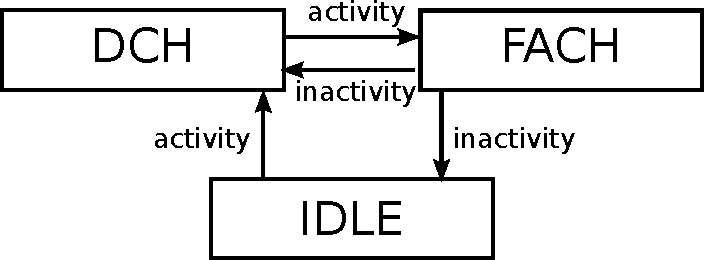
\includegraphics[width=0.8\columnwidth]{images/rrc-simplified-state-model.pdf}
	\caption{Simplified \gls{RRC} State Model.}
	\label{c4:fig:rrcstatemodel}
\end{figure}


As indicated before, most nodes in a cellular mobile network keep all sorts of states characterizing the data connection. For the tunnel management aspects, two state machines are of special note.

\begin{figure}[htb]
	\centering
	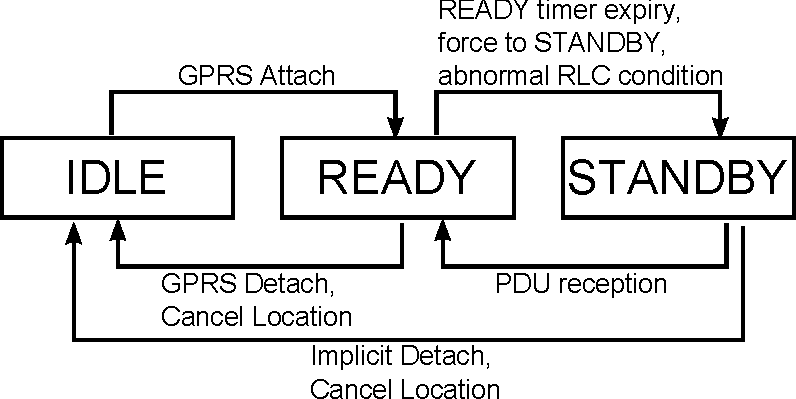
\includegraphics[width=0.8\columnwidth]{images/mm-state-model.pdf}
	\caption{\gls{SGSN} Mobility Management State Model.}
	\label{c4:fig:mmstatemodel}
\end{figure}

First, consider the Mobility Management state machine depicted in Figure \ref{c4:fig:mmstatemodel}, defined in \cite{3gpp.23.060}, and held in both the \gls{SGSN} as well as the mobile device. It describes the general state of the data connection, and switches states based either on an idle timer, or when new packets arrive for the mobile device. Therefore, it also controls tunnel management, as the involved \gls{GPRS} Detach and Attach procedures involve deleting and creating contexts. We identify user traffic dynamics as one vector to influence core network signaling, similar to the observations in \cite{lee2007detection}.


The \gls{RRC} state machine shown in Figure \ref{c4:fig:rrcstatemodel} governs the usage of radio channels, i.e. spectral and temporal usage of the wireless interface. State changes happen depending on the inter-arrival time of user packets. In this case, if the state machine transitions to the IDLE state, the \gls{RAB} on the path between mobile device and \gls{SGSN} is not needed anymore and will be deleted, in most cases destroying the \gls{SGSN} and \gls{GGSN} \gls{PDP} Context as well.

%\subsection{Network State and State Exchange}
per \gls{PLMN} node, cf. \gls{3GPP} \gls{TS} 23.401 clause 5.7.


% TODO: convert to UMTS

% \begin{figure}[htb]
% 	\centering
% 	\includegraphics[width=1.0\textwidth]{images/UE-requested-PDN-connectivity.pdf}
% mdcm	\caption{\gls{PDN} connectivity request by the UE procedure sequence diagram.}
% 	\label{c4:fig:3gpp-uepdnreq}
% \end{figure}



%%%%%%%%%%%%%%%%%%%%%%%%%%%%%%%%%%%%%%%%%%%%%%%%%%%%%%%%%%%%%%%%%%%%%%%%%%%%%%%%
\paragraph{Discussion of \texorpdfstring{\acrshort{gtp}}{GTP} Signaling}

Looking at the Create, Update and Delete PDP Context Request and Reply message pairs we can already directly deduce some possibly load-related information. The total tunnel duration originates from the time delta between corresponding Create and Delete events. The shorter those tunnels are the higher will be volume of signaling messages and the necessary processing for these messages. Conversely, longer tunnel durations cause an increased overall memory footprint in the involved nodes to store the \gls{PDP} Contexts. Large numbers of update messages, especially combined with frequent \gls{RAT} switches, are usually an indicator for highly mobile devices switching their routing area. 
The time between a request and its corresponding response could also be an indicator for the amount of processing involved for this message as well as the current general processing load at the \gls{GGSN}.

As discussed, most of the actions in the network as well as in the mobile devices are reflected in the presented tunnel management messaging. Therefore, taking a look at the dynamics of this control aspect in real networks gives valuable insights on the influence of many of the networks' aspects.

Looking at the Create, Update and Delete \gls{PDP} Context Request and Reply message pairs we can already deduce a certain amount of information. Measuring the time delta between corresponding Create and Delete events obviously gives the total duration a tunnel was established. Given the amount of user-plane IP traffic transferred, when the tunnel durations are short, we can expect the number of tunnel creation and deletion events to go up instead, resulting in a higher volume of signaling messages and an increase in processing for these messages. Conversely, longer tunnel durations cause an increased overall memory footprint in the involved nodes to store the \gls{PDP} Contexts. Large numbers of update messages, especially combined with frequent \gls{RAT} switches, are usually an indicator for highly mobile devices switching their routing area. This mobility behavior could be investigated by evaluating the update messages.

As discussed, most of the actions in the network as well as in the mobile devices are reflected in the presented tunnel management messaging. Therefore, taking a look at the dynamics of this control aspect in real networks gives valuable insights on the influence of many of the networks' aspects.




% \subsubsection{Information Elements Wire Format}

% \paragraph{IMSI}

% \begin{table}[htb]
% 	\caption{IMSI Information Element Format.}
% 	\label{c4:tbl:imsiieformat}
% 	\begin{tabu}{X[c]|X|X|X|X|X|X|X|X|}
% 	\multicolumn{1}{c}{} & \multicolumn{8}{c}{\textbf{Bits}} \\
% 	\cline{2-9} \textbf{Octets} & 8 & 7 & 6 & 5 & 4 & 3 & 2 & 1 \\ 
% 	\cline{2-9} 1 & \multicolumn{8}{c|}{Type = 1 (decimal)} \\ 
% 	\cline{2-9} 2 to 3 & \multicolumn{8}{c|}{Length = n}  \\ 
% 	\cline{2-9} 4 & \multicolumn{4}{c|}{Spare} & \multicolumn{4}{c|}{Instance} \\ 
% 	\cline{2-9} 5 & \multicolumn{4}{c|}{Number digit 2} & \multicolumn{4}{c|}{Number digit 1} \\ 
% 	\cline{2-9} 6 & \multicolumn{4}{c|}{Number digit 4} & \multicolumn{4}{c|}{Number digit 3} \\ 
% 	\cline{2-9} ... & \multicolumn{4}{c|}{...} & \multicolumn{4}{c|}{...} \\ 
% 	\cline{2-9} n+4 & \multicolumn{4}{c|}{Number digit m} & \multicolumn{4}{c|}{Number digit m-1} \\ 
% 	\cline{2-9}
% 	\end{tabu}
% \end{table}

% Decimals coded as TBCD; if odd number fill last nibble with 1; max digits is 15.\\
% Max IE size 12 Byte.

% \paragraph{APN}

% \begin{table}[htb]
% 	\caption{APN Information Element Format.}
% 	\label{c4:tbl:apnieformat}
% 	\begin{tabu}{X[c]|X|X|X|X|X|X|X|X|}
% 	\multicolumn{1}{c}{} & \multicolumn{8}{c}{\textbf{Bits}} \\
% 	\cline{2-9} \textbf{Octets} & 8 & 7 & 6 & 5 & 4 & 3 & 2 & 1 \\ 
% 	\cline{2-9} 1 & \multicolumn{8}{c|}{Type = 71 (decimal)} \\ 
% 	\cline{2-9} 2 to 3 & \multicolumn{8}{c|}{Length = n}  \\ 
% 	\cline{2-9} 4 & \multicolumn{4}{c|}{Spare} & \multicolumn{4}{c|}{Instance} \\ 
% 	\cline{2-9} 5 to (n+4) & \multicolumn{8}{c|}{Access Point Name} \\ 
% 	\cline{2-9}
% 	\end{tabu} 
% \end{table}

% Full APN name including APN Network Identifier and APN Operator Identifier.
% Network Identifier: max length 63 bytes.
% Operator Identifier: mnc<3digits>.mcc<3digits>.gprs; 16 bytes (18 incl dots).
% (Ex: ggsn-cluster-A.provinceB.mnc012.mcc345.gprs)

% Max total $4+63+16=83$

% \paragraph{AMBR}

% \begin{table}[htb]
% 	\caption{APN Information Element Format.}
% 	\label{c4:tbl:abmrieformat}
% 	\begin{tabu}{X[c]|X|X|X|X|X|X|X|X|}
% 	\multicolumn{1}{c}{} & \multicolumn{8}{c}{\textbf{Bits}} \\
% 	\cline{2-9} \textbf{Octets} & 8 & 7 & 6 & 5 & 4 & 3 & 2 & 1 \\ 
% 	\cline{2-9} 1 & \multicolumn{8}{c|}{Type = 72 (decimal)} \\ 
% 	\cline{2-9} 2 to 3 & \multicolumn{8}{c|}{Length = n}  \\ 
% 	\cline{2-9} 4 & \multicolumn{4}{c|}{Spare} & \multicolumn{4}{c|}{Instance} \\ 
% 	\cline{2-9} 5 to 8 & \multicolumn{8}{c|}{APN-AMBR for uplink} \\ 
% 	\cline{2-9} 9 to 12 & \multicolumn{8}{c|}{APN-AMBR for downlink} \\ 
% 	\cline{2-9}
% 	\end{tabu} 
% \end{table}

% Total size 12 bytes.


% \paragraph{Recovery}

% \begin{table}[htb]
% 	\caption{Recovery Information Element Format.}
% 	\label{c4:tbl:recoveryieformat}
% 	\begin{tabu}{X[c]|X|X|X|X|X|X|X|X|}
% 	\multicolumn{1}{c}{} & \multicolumn{8}{c}{\textbf{Bits}} \\
% 	\cline{2-9} \textbf{Octets} & 8 & 7 & 6 & 5 & 4 & 3 & 2 & 1 \\ 
% 	\cline{2-9} 1 & \multicolumn{8}{c|}{Type = 3 (decimal)} \\ 
% 	\cline{2-9} 2 to 3 & \multicolumn{8}{c|}{Length = n}  \\ 
% 	\cline{2-9} 4 & \multicolumn{4}{c|}{Spare} & \multicolumn{4}{c|}{Instance} \\ 
% 	\cline{2-9} 5 to (n+4) & \multicolumn{8}{c|}{Recovery (Restart Counter} \\ 
% 	\cline{2-9}
% 	\end{tabu} 
% \end{table}

% IN GTPv2 first release IE length is 5 bytes. May be longer in the future.


% \paragraph{MEI}

% \begin{table}[htb]
% 	\caption{MEI Information Element Format.}
% 	\label{c4:tbl:meiieformat}
% 	\begin{tabu}{X[c]|X|X|X|X|X|X|X|X|}
% 	\multicolumn{1}{c}{} & \multicolumn{8}{c}{\textbf{Bits}} \\
% 	\cline{2-9} \textbf{Octets} & 8 & 7 & 6 & 5 & 4 & 3 & 2 & 1 \\ 
% 	\cline{2-9} 1 & \multicolumn{8}{c|}{Type = 75 (decimal)} \\ 
% 	\cline{2-9} 2 to 3 & \multicolumn{8}{c|}{Length = n}  \\ 
% 	\cline{2-9} 4 & \multicolumn{4}{c|}{Spare} & \multicolumn{4}{c|}{Instance} \\ 
% 	\cline{2-9} 5 to (n+4) & \multicolumn{8}{c|}{Mobile Equipment (ME) Identity} \\ 
% 	\cline{2-9}
% 	\end{tabu}
% \end{table}

% 15 (IMEI) or 16 (IMEISV) BCD digits filled with 1 to full octet. Size is 12 bytes.

% \paragraph{MSISDN}

% \begin{table}[htb]
% 	\caption{MSISDN Information Element Format.}
% 	\label{c4:tbl:msisdnieformat}
% 	\begin{tabu}{X[c]|X|X|X|X|X|X|X|X|}
% 	\multicolumn{1}{c}{} & \multicolumn{8}{c}{\textbf{Bits}} \\
% 	\cline{2-9} \textbf{Octets} & 8 & 7 & 6 & 5 & 4 & 3 & 2 & 1 \\ 
% 	\cline{2-9} 1 & \multicolumn{8}{c|}{Type = 76 (decimal)} \\ 
% 	\cline{2-9} 2 to 3 & \multicolumn{8}{c|}{Length = n}  \\ 
% 	\cline{2-9} 4 & \multicolumn{4}{c|}{Spare} & \multicolumn{4}{c|}{Instance} \\ 
% 	\cline{2-9} 5 & \multicolumn{4}{c|}{Number digit 2} & \multicolumn{4}{c|}{Number digit 1} \\ 
% 	\cline{2-9} 6 & \multicolumn{4}{c|}{Number digit 4} & \multicolumn{4}{c|}{Number digit 3} \\ 
% 	\cline{2-9} ... & \multicolumn{4}{c|}{...} & \multicolumn{4}{c|}{...} \\ 
% 	\cline{2-9} n+4 & \multicolumn{4}{c|}{Number digit m} & \multicolumn{4}{c|}{Number digit m-1} \\ 
% 	\cline{2-9}
% 	\end{tabu}
% \end{table}

% MSISDN limited to 15 digits. Max total size 12 bytes.


% \paragraph{Indication}

% \begin{table}[htb]
% 	\caption{Indication Information Element Format.}
% 	\label{c4:tbl:indicationieformat}
% 	\begin{tabu}{X[c]|X|X|X|X|X|X|X|X|}
% 	\multicolumn{1}{c}{} & \multicolumn{8}{c}{\textbf{Bits}} \\
% 	\cline{2-9} \textbf{Octets} & 8 & 7 & 6 & 5 & 4 & 3 & 2 & 1 \\ 
% 	\cline{2-9} 1 & \multicolumn{8}{c|}{Type = 77 (decimal)} \\ 
% 	\cline{2-9} 2 to 3 & \multicolumn{8}{c|}{Length = n}  \\ 
% 	\cline{2-9} 4 & \multicolumn{4}{c|}{Spare} & \multicolumn{4}{c|}{Instance} \\ 
% 	\cline{2-9} 5 & DAF & DTF & HI & DFI & OI & ISRSI & ISRAI & SGWCI \\ 
% 	\cline{2-9} 6 & Spare & UIMSI & CFSI & CRSI & P & PT & SI & MSV \\ 
% 	\cline{2-9} 7 to (n+4) & \multicolumn{8}{c|}{These octet(s) is/are present only if explicitly specified} \\ 
% 	\cline{2-9}
% 	\end{tabu}
% \end{table}

% Size is 7 bytes.

% \paragraph{PCO}


% \begin{table}[htb]
% 	\caption{PCO Information Element Format.}
% 	\label{c4:tbl:pcoieformat}
% 	\begin{tabu}{X[c]|X|X|X|X|X|X|X|X|}
% 	\multicolumn{1}{c}{} & \multicolumn{8}{c}{\textbf{Bits}} \\
% 	\cline{2-9} \textbf{Octets} & 8 & 7 & 6 & 5 & 4 & 3 & 2 & 1 \\ 
% 	\cline{2-9} 1 & \multicolumn{8}{c|}{Type = 78 (decimal)} \\ 
% 	\cline{2-9} 2 to 3 & \multicolumn{8}{c|}{Length = n}  \\ 
% 	\cline{2-9} 4 & \multicolumn{4}{c|}{Spare} & \multicolumn{4}{c|}{Instance} \\ 
% 	\cline{2-9} 5 to (n+4) & \multicolumn{8}{c|}{Protocol Configuration Options} \\
% 	\cline{2-9}
% 	\end{tabu}
% \end{table}

% Minimum length 4+3-3, maximum length 4+253-3; average?


% \paragraph{PAA}

% \begin{table}[htb]
% 	\caption{PAA Information Element Format.}
% 	\label{c4:tbl:paaieformat}
% 	\begin{tabu}{X[c]|X|X|X|X|X|X|X|X|}
% 	\multicolumn{1}{c}{} & \multicolumn{8}{c}{\textbf{Bits}} \\
% 	\cline{2-9} \textbf{Octets} & 8 & 7 & 6 & 5 & 4 & 3 & 2 & 1 \\ 
% 	\cline{2-9} 1 & \multicolumn{8}{c|}{Type = 79 (decimal)} \\ 
% 	\cline{2-9} 2 to 3 & \multicolumn{8}{c|}{Length = n}  \\ 
% 	\cline{2-9} 4 & \multicolumn{4}{c|}{Spare} & \multicolumn{4}{c|}{Instance} \\ 
% 	\cline{2-9} 5 & \multicolumn{5}{c|}{Spare} & \multicolumn{3}{c|}{PDN Type} \\
% 	\cline{2-9} 6 to (n+4) & \multicolumn{8}{c|}{PDN Adress and Prefix} \\
% 	\cline{2-9}
% 	\end{tabu} 
% \end{table}

% Either 9 (IPv4), 22 (IPv6), or 26 (IPv4v6).


% \paragraph{RAT Type}


% \begin{table}[htb]
% 	\caption{RAT Information Element Format.}
% 	\label{c4:tbl:ratieformat}
% 	\begin{tabu}{X[c]|X|X|X|X|X|X|X|X|}
% 	\multicolumn{1}{c}{} & \multicolumn{8}{c}{\textbf{Bits}} \\
% 	\cline{2-9} \textbf{Octets} & 8 & 7 & 6 & 5 & 4 & 3 & 2 & 1 \\ 
% 	\cline{2-9} 1 & \multicolumn{8}{c|}{Type = 82 (decimal)} \\ 
% 	\cline{2-9} 2 to 3 & \multicolumn{8}{c|}{Length = n}  \\ 
% 	\cline{2-9} 4 & \multicolumn{4}{c|}{Spare} & \multicolumn{4}{c|}{Instance} \\ 
% 	\cline{2-9} 5 & \multicolumn{8}{c|}{RAT Type} \\
% 	\cline{2-9} 6 to (n+4) & \multicolumn{8}{c|}{These octet(s) is/are present only if explicitly specified} \\
% 	\cline{2-9}
% 	\end{tabu} 
% \end{table}

% Maximum length 5 to ?.

% \paragraph{Serving Network}

% \begin{table}[htb]
% 	\caption{Serving Network Information Element Format.}
% 	\label{c4:tbl:servingnetieformat}
% 	\begin{tabu}{X[c]|X|X|X|X|X|X|X|X|}
% 	\multicolumn{1}{c}{} & \multicolumn{8}{c}{\textbf{Bits}} \\
% 	\cline{2-9} \textbf{Octets} & 8 & 7 & 6 & 5 & 4 & 3 & 2 & 1 \\ 
% 	\cline{2-9} 1 & \multicolumn{8}{c|}{Type = 83 (decimal)} \\ 
% 	\cline{2-9} 2 to 3 & \multicolumn{8}{c|}{Length = n}  \\ 
% 	\cline{2-9} 4 & \multicolumn{4}{c|}{Spare} & \multicolumn{4}{c|}{Instance} \\ 
% 	\cline{2-9} 5 & \multicolumn{4}{c|}{MCC digit 2} & \multicolumn{4}{c|}{MCC digit 1} \\ 
% 	\cline{2-9} 6 & \multicolumn{4}{c|}{MNC digit 3} & \multicolumn{4}{c|}{MCC digit 3} \\ 
% 	\cline{2-9} 7 & \multicolumn{4}{c|}{MNC digit 2} & \multicolumn{4}{c|}{MNC digit 1} \\ 
% 	\cline{2-9} 8 to (n+4) & \multicolumn{8}{c|}{These octet(s) is/are present only if explicitly specified} \\
% 	\cline{2-9}
% 	\end{tabu}
% \end{table} 

% Maximum length 7 to ?.


% \paragraph{User Location Information}

% \begin{table}[htb]
% 	\caption{User Location Information Element Format.}
% 	\label{c4:tbl:userlocieformat}
% 	\begin{tabu}{X[c]|X|X|X|X|X|X|X|X|}
% 	\multicolumn{1}{c}{} & \multicolumn{8}{c}{\textbf{Bits}} \\
% 	\cline{2-9} \textbf{Octets} & 8 & 7 & 6 & 5 & 4 & 3 & 2 & 1 \\ 
% 	\cline{2-9} 1 & \multicolumn{8}{c|}{Type = 86 (decimal)} \\ 
% 	\cline{2-9} 2 to 3 & \multicolumn{8}{c|}{Length = n}  \\ 
% 	\cline{2-9} 4 & \multicolumn{4}{c|}{Spare} & \multicolumn{4}{c|}{Instance} \\ 
% 	\cline{2-9} 5 & \multicolumn{3}{c|}{Spare} & ECGI & TAI & RAI & SAI & CGI \\ 
% 	\cline{2-9} a to a+6 & \multicolumn{8}{c|}{CGI} \\ 
% 	\cline{2-9} 7 & \multicolumn{8}{c|}{SAI} \\ 
% 	\cline{2-9} 7 & \multicolumn{8}{c|}{RAI} \\ 
% 	\cline{2-9} 7 & \multicolumn{8}{c|}{TAI} \\ 
% 	\cline{2-9} 7 & \multicolumn{8}{c|}{ECGI} \\ 
% 	\cline{2-9} 8 to (n+4) & \multicolumn{8}{c|}{These octet(s) is/are present only if explicitly specified} \\
% 	\cline{2-9}
% 	\end{tabu} 
% \end{table}



% Information Elements Table for PDP Context Activation Case only for GTPv2 (LTE)
% \begin{longtabu} to\linewidth{| X[2,l] | X[2,c] | X[l] | X[4] |}
% \hline
% Information Element 						& IE Type 					& Max Wire Size (Bytes)	& Comment \\ \hline
% \gls{IMSI} 										& IMSI 						& 12					& \\ \hline
% \gls{MSISDN} 										& MSISDN					& 12					& On S11 Interface if provided by HSS; In case of UE requested connectivity if MME has it stored. \\ \hline
% MEI Identity 								& MEI 						& 12					& If available at MME. \\ \hline
% User Location Information 					& ULI						& 						& E-UTRAN initial attach \&  UE requested connectivity only; included by S-GW if received from MME via S5/S8; included on S4 and S5/S8 for PDP context activation, either CGI, SAI, or RAI. \\ \hline
% Serving Network								& Serving Network			& 						& Initial E-UTRAN attach, context activation and UE requested connectivity \\ \hline
% \gls{RAT} Type									& RAT Type					& 5						& \\ \hline
% Indication Flags							& Indication				& 6						& Flags: S5/S8 Protocol Type; Dual Address Bearer Flag; Handover Indication; Direct Tunnel Flag; Piggybacking Supported; Change Reporting Support Indication \\ \hline
% Sender F-TEID for Control Plane				& F-TEID					& 						& \\ \hline
% P-G S5/S8 Address for Control Plane or PMIP	& F-TEID					& 						& On S11/S4 interfaces; 0 if initial attach, context activation or PDN connectivity \\ \hline
% Access Point Name							& APN						& 83					& \\ \hline
% Selection Mode								& Selection Mode			& 						& Indicate whether subscribed or non-subscribed, chosen by MME, was selected \\ \hline
% PDN Type									& PDN Type					& 						& IPv4, IPv6 or IPv4v6. \\ \hline
% PDN Address Allocation						& PAA						& 26					& Set to static IP address; else (dynamic) to 0.0.0.0 or IPv6 Prefix Length 0. \\ \hline
% Maximum APN Restriction						& APN Restriction			& 						& Set to most stringent restriction of any active bearer. \\ \hline
% Aggregate Maximum Bit Rate					& ABMR						& 12					& \\ \hline
% Protocol Configuration Options				& PCO						& 254					& Forwarded from UE to P-GW via S-GW via MME. \\ \hline
% Bearer Contexts to be created				& Bearer Context			& 						& present multiple times to represent list of bearers \\ \hline
% Trace Information							& Trace Information 		& 						& If S-GW / P-GW is activated. \\ \hline
% Recovery									& Recovery					& 5						& If peer node contacted for the first time. \\ \hline
% MME-FQ-CSID									& FQ-CSID					& 						& Included by MME on S11 \\ \hline
% SGW-FQ-CSID									& FQ-CSID					& 						& Included by SGW on S5/S8 \\ \hline
% UE Time Zone								& UE Time Zone 				& 						& Can be included by MME on S11; forwarded to P-GW via S-GW \\ \hline
% User CSG Information						& UCI						& 						& If \gls{UE} accessed via CSG cell or hybrid cell \\ \hline
% Charging Characteristics					& Charging Characteristics	&						& \\ \hline
% Private Extensions							& Private Extensions		&						& \\ \hline
% \end{longtabu}





% \begin{figure}[htb]
% 	\centering
%  	\includegraphics[width=0.9\textwidth]{images/eNB-MME-layers.pdf}
%  	\caption{Control plane protocol stack at the S1-MME interface between eNodeB and MME.}
%  	\label{c4:fig:stack-enbmme}
% \end{figure}

% \begin{figure}[htb]
% 	 \centering
% 	 \includegraphics[width=0.9\textwidth]{images/SGSN-MME-layers.pdf}
% 	 \caption{Control plane protocol stack at the S3 interface between SGSN and MME.}
% 	 \label{c4:fig:stack-sgsnmme}
% \end{figure}

% \begin{figure}[htb]
% 	\centering
% 	\includegraphics[width=0.9\textwidth]{images/S-GW-P-GW-layers.pdf}
% 	\caption{Optional control plane protocol stack at the S5 interface between SGW and PGW.}
% 	\label{c4:fig:stack-sgwpgw}
% \end{figure}

% \begin{figure}[htb]
% 	\centering
% 	\includegraphics[width=0.9\textwidth]{images/MME-S-GW-layers.pdf}
% 	\caption{Control plane protocol stack at the S11 interface between MME and SGW.}
% 	\label{c4:fig:stack-mmesgw}
% \end{figure}



%List of interfaces in the 3G/LTE PS network
%\begin{itemize}
%\item \textbf{Uu}: Interface between the mobile station (MS) and the fixed network part in Iu mode. The Uu interface is the Iu mode network interface for providing packet data services over the radio to the MS. The MT part of the MS is used to access the UMTS services through this interface.
%\item \textbf{Iub}: Interface between a NodeB and a RNC.
%\item \textbf{IuPS}: Interface between a RNC and a SGSN.
%\item \textbf{S1-U}: Interface between a eNodeB and a S-GW. User plane bearer tunneling.
% \item \textbf{S1-MME}: Interface between a eNodeB and a MME.
% \item \textbf{S3}: Interface between a SGSN and a MME. User/bearer information exchange for active/idle state 3g network access mobility.
% \item \textbf{S4}: Interface between a SGSN and a S-GW.	 2G user plane tunneling. GPRS mobility and control.
% \item \textbf{S5}: Interface between a S-GW and a P-GW within the same PLMN. User plane tunneling; S-GW relocation due to mobility.
% \item \textbf{S6a}: Interface between a MME and a HSS. Auth/auth data transfer to evolved system.
% \item \textbf{Gr/S6d}: Interface between a SGSN and a HSS. 
% \item \textbf{S8}: Interface between a S-GW and a P-GW in different PLMNs. Inter-PLMN variant to S5.
% \item \textbf{S9}: Interface between a PRCF and the packet data network. Data exchange to visited PCRF PLMN.
% \item \textbf{S11}: Interface between a S-GW and a MME.
% \item \textbf{S12}: UTRAN to S-GW reference point. Based on Iu-u/Gn-u. Direct Tunnel via GTP-U.
% \item \textbf{S13}: Interface between a MME and a EIR. UE identity check.
% \item \textbf{SGi}: The reference point between the EPC based PLMN and the packet data network. Same as Gi for 3gpp.

% \item \textbf{GC}: Interface between a HSS and a GGSN.
% \item \textbf{Gf}: Interface between a SGSN and a EIR.
% \item \textbf{Gi}: Reference point between Packet Domain and an external packet data network.
% \item \textbf{Gn}: Interface between two GSNs within the same PLMN.
% \item \textbf{Gp}: Interface between two GSNs in different PLMNs. The Gp interface allows support of Packet Domain network services across areas served by the co-operating PLMNs.
% \item \textbf{Gx}: Interface between a PCRF and a P-GW/GGSN. QoS policy and charging rules transfer.
% \item \textbf{Gxc}: Interface between a PCRF and a S-GW.

% \item \textbf{Rx}: Interface between a PRCF and the packet data network.
% \end{itemize}


%EMM Service request procedure
% \begin{figure}[htb]
% 	\centering
% 	\includegraphics[width=1.0\textwidth]{images/UE-service-request.pdf}
% 	\caption{EMM service request procedure sequence diagram.}
% 	\label{c4:fig:3gpp-ueservicereq}
% \end{figure}

% Annotations:
% 1. Encapsulated in RRC message.
% 2. Forwarded in S1-AP Initial UE Message.
% 3. Various security procedures.

%	25.401 \cite{3gpp.25.401} UTRAN overall description
%	25.931 \cite{3gpp.25.931} UTRAN functions, examples on signalling procedures
%	23.401 \cite{3gpp.23.401} \gls{E-UTRAN} procedures (LTE only)
%	24.007 \cite{3gpp.24.007} radio interface signaling % only Um interface in plain GSM/GPRS
%	36.300 \cite{3gpp.36.300} \gls{E-UTRAN} description (LTE only) 
%	36.414 \cite{3gpp.36.414} Evolved Universal Terrestrial Radio Access Network (E-UTRAN); S1 data transport (radio bearer)
%	22.060 \cite{3gpp.22.060} basic and short \gls{GPRS} service description; unchanged since Release 6 (2004)
%	23.060 \cite{3gpp.23.060} \gls{GPRS} description : \gls{GPRS} specific procedures, interfaces and nodes; mobility management; radio management; packet routing; operational aspects



	%23.402 \cite{3gpp.23.402} (LTE only) non-\gls{3GPP} accesses
	%24.301 \cite{3gpp.24.301} EPS Non-Access-Stratum protocol between UE and MME on Uu

% Relevant protocols and interfaces between nodes:
% \begin{itemize}
% 	\item \gls{gtp}, \gls{gtpv2}, GTP-u, GTP-c, \gls{SGSN} to \gls{GGSN} and others (specify!), on top of \gls{UDP}, GTPv1 will be described in detail in a separate section as it is at the core of the upcoming investigations.
% 	\item \gls{MAP} / \gls{SS7}: \gls{SGSN} - \gls{HLR}, \gls{GGSN} - \gls{HLR} and others; subscriber management and information exchange
% 	\item Diameter \cite{rfc6733}: \gls{MME} - \gls{HSS}, \gls{SGSN} - \gls{HSS}, replacement for \gls{MAP}, subscriber management

% 	\item PMIPv6 on \gls{SGW} - \gls{PGW}, alternative tunneling protocol to GTPv2
% \end{itemize}


%%%%%%%%%%%%%%%%%%%%%%%%%%%%%%%%%%%%%%%%%%%%%%%%%%%%%%%%%%%%%%%%%%%%%%%%%%%%%%%%
%%!TEX root = dissertation.tex
%%%%%%%%%%%%%%%%%%%%%%%%%%%%%%%%%%%%%%%%%%%%%%%%%%%%%%%%%%%%%%%%%%%%%%%%%%%%%%%%
%
% Collection of all relevant mobile radio specifications and descriptions
%
\section{Übersicht}

\begin{itemize}
\item Einarbeitung
	\begin{itemize}
		\item Architektur von 3G-Netzen
		\item Modelle zur Beschreibung von Datenverkehrsflüssen
		\item Einarbeitung in das Messsystem des FTW
	\end{itemize}
\item Definition eines einfachen Bearer-Modells
\item Programmierung der Auswertung
\item Durchführung und Auswertung der Messungen
\item Anfertigung eines Berichtes
\end{itemize}

\section{Modeling}
Macroscopic Behavior

	-- time Connection Setup until Call Termination with Talk Spurts
	--> ON/OFF Process
	--> Empricial measurement
	
Source Traffic Model
	-- 2 parts: 
		arrival process for user activities
		process describing activity phase
	-- arrival time:
		User begins web browsing
	
Simulation \& Software
	ns-2 UMTS mobile parts only
	ns-3 GSoC2010 implementing \ac{UTRAN} (MAC\&PHY) incl radio bearers (+OpenFlow)
	Harald Welte GPRS: OpenBSC, OpenGGSN incl GTP
	

EPS first introduced in 3GPP Release 8, completed in March 2009. Consisting of EUTRAN, EPC (formerly SAE)


	


\begin{figure}[htbp]
 \centering
 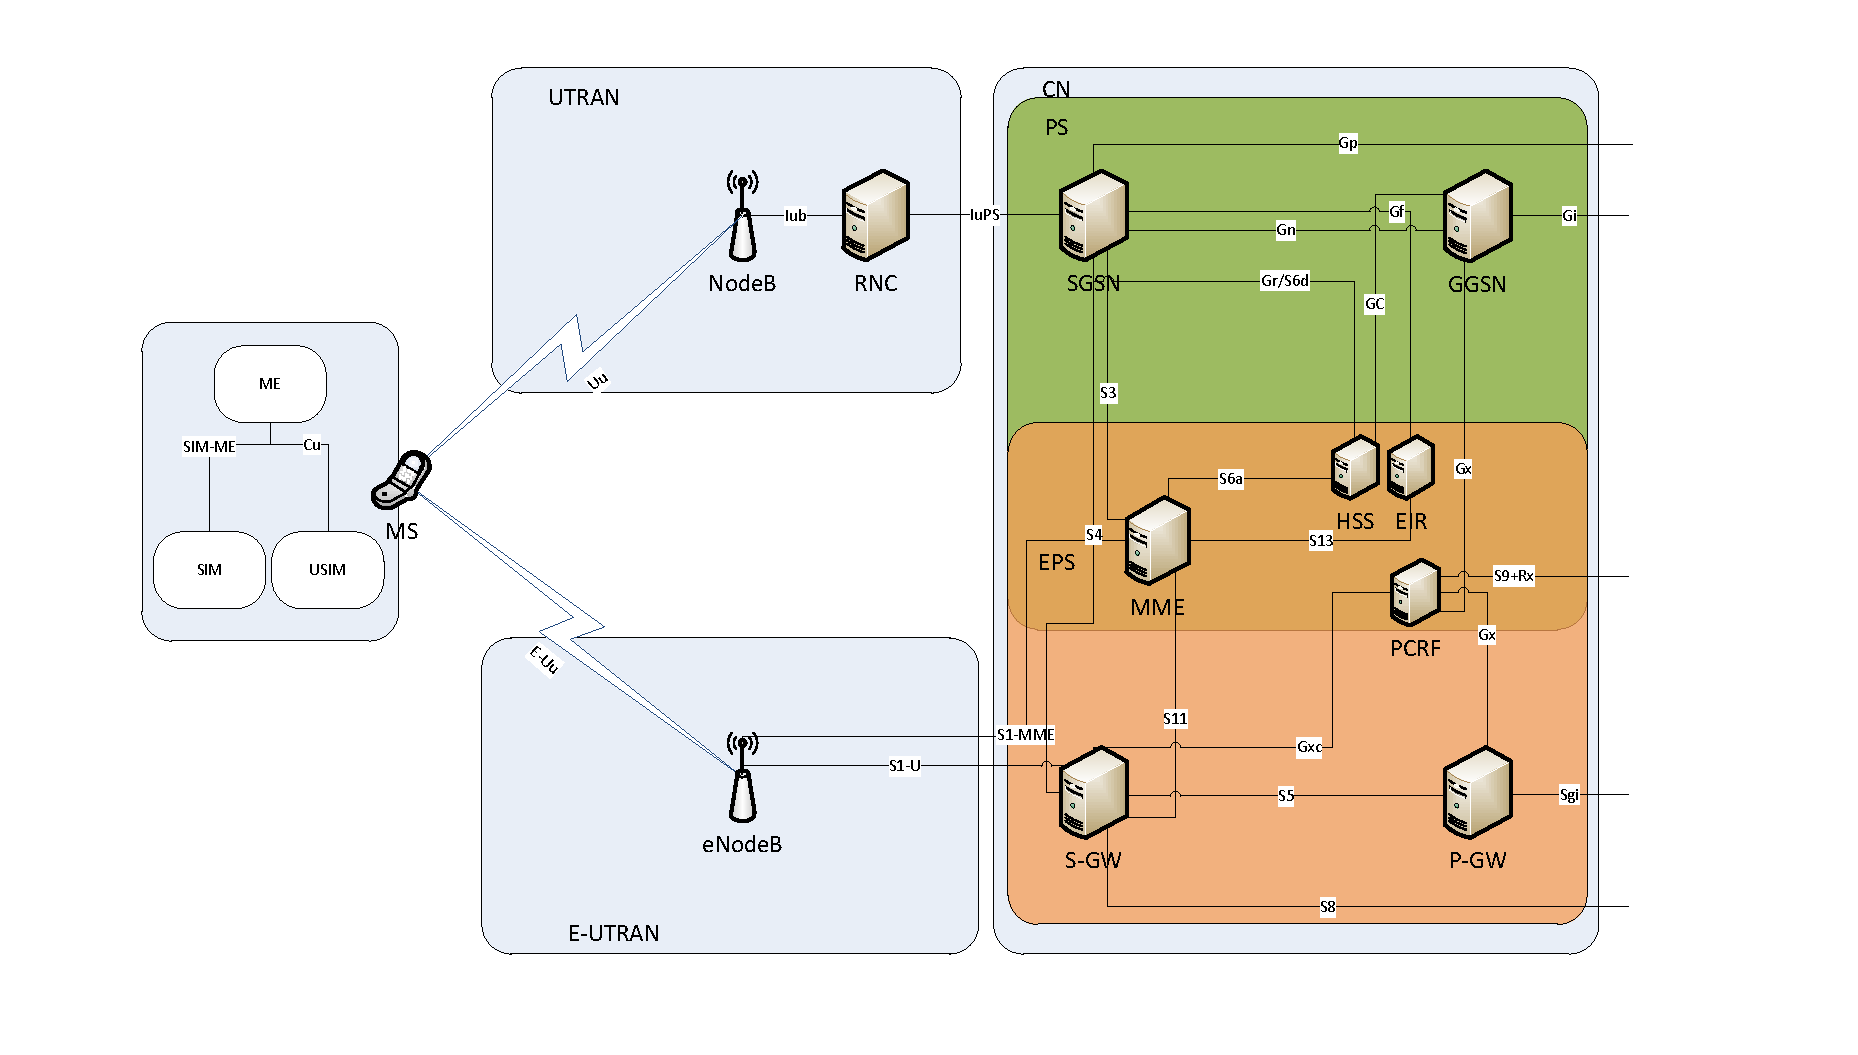
\includegraphics[width=1.0\textwidth]{images/3gpp/eps_ps-overview.pdf}
 \caption{Beispielnetz}\label{fig:netzwerk2}
\end{figure}

List of interfaces in the 3G/LTE PS network
\begin{itemize}
\item \textbf{Uu}: Interface between the mobile station (MS) and the fixed network part in Iu mode. The Uu interface is the Iu mode network interface for providing packet data services over the radio to the MS. The MT part of the MS is used to access the UMTS services through this interface.
\item \textbf{Iub}: Interface between a NodeB and a RNC.
\item \textbf{IuPS}: Interface between a RNC and a SGSN.

\item \textbf{S1-U}: Interface between a eNodeB and a S-GW. User plane bearer tunneling.
\item \textbf{S1-MME}: Interface between a eNodeB and a MME.
\item \textbf{S3}: Interface between a SGSN and a MME. User/bearer information exchange for active/idle state 3g network access mobility.
\item \textbf{S4}: Interface between a SGSN and a S-GW.	 2G user plane tunneling. GPRS mobility and control.
\item \textbf{S5}: Interface between a S-GW and a P-GW within the same PLMN. User plane tunneling; S-GW relocation due to mobility.
\item \textbf{S6a}: Interface between a MME and a HSS. Auth/auth data transfer to evolved system.
\item \textbf{Gr/S6d}: Interface between a SGSN and a HSS. 
\item \textbf{S8}: Interface between a S-GW and a P-GW in different PLMNs. Inter-PLMN variant to S5.
\item \textbf{S9}: Interface between a PRCF and the packet data network. Data exchange to visited PCRF PLMN.
\item \textbf{S11}: Interface between a S-GW and a MME.
\item \textbf{S12}: UTRAN to S-GW reference point. Based on Iu-u/Gn-u. Direct Tunnel via GTP-U.
\item \textbf{S13}: Interface between a MME and a EIR. UE identity check.
\item \textbf{SGi}: The reference point between the EPC based PLMN and the packet data network. Same as Gi for 3gpp.

\item \textbf{GC}: Interface between a HSS and a GGSN.
\item \textbf{Gf}: Interface between a SGSN and a EIR.
\item \textbf{Gi}: Reference point between Packet Domain and an external packet data network.
\item \textbf{Gn}: Interface between two GSNs within the same PLMN.
\item \textbf{Gp}: Interface between two GSNs in different PLMNs. The Gp interface allows support of Packet Domain network services across areas served by the co-operating PLMNs.
\item \textbf{Gx}: Interface between a PCRF and a P-GW/GGSN. QoS policy and charging rules transfer.
\item \textbf{Gxc}: Interface between a PCRF and a S-GW.

\item \textbf{Rx}: Interface between a PRCF and the packet data network.
\end{itemize}

\section{Control Plane Protocol Stacks}

\begin{figure}[htbp]
 \centering
 \includegraphics[width=1.0\textwidth]{images/3gpp/eNB-MME-layers.pdf}
 \caption{Beispielnetz}\label{fig:3gpp-enbmme}
\end{figure}

\begin{figure}[htbp]
 \centering
 \includegraphics[width=1.0\textwidth]{images/3gpp/SGSN-MME-layers.pdf}
 \caption{Beispielnetz}\label{fig:3gpp-sgsnmme}
\end{figure}

\begin{figure}[htbp]
 \centering
 \includegraphics[width=1.0\textwidth]{images/3gpp/S-GW-P-GW-layers.pdf}
 \caption{Beispielnetz}\label{fig:3gpp-sgwpgw}
\end{figure}

\begin{figure}[htbp]
 \centering
 \includegraphics[width=1.0\textwidth]{images/3gpp/MME-S-GW-layers.pdf}
 \caption{Beispielnetz}\label{fig:3gpp-mmesgw}
\end{figure}


\begin{figure}[htbp]
 \centering
 \includegraphics[width=1.0\textwidth]{images/3gpp/3g-userplane.pdf}
 \caption{Beispielnetz}\label{fig:3gpp-umtsuserplane}
\end{figure}

\begin{figure}[htbp]
 \centering
 \includegraphics[width=1.0\textwidth]{images/3gpp/LTE-userplane.pdf}
 \caption{Beispielnetz}\label{fig:3gpp-lteuserplane}
\end{figure}


\section{Bearers}

As you said only 11 bearer are permitted.
So PDN connection(Default bearer) + Dedicated bearers put together should not exceed 11 bearers at any instant of time at UE side.
Theoretically 11 PDN connections are possible. But i dont think it will be of any use in practical EPS topology.

One UE Can have Maximum 3 PDN connection.
where as my knowledge is concern one UE can support maximum 11 bearers, 3 default and 8 dedicated bearers.

Does I will get in any spec for this. As the default bearer are of  NON-GBR type and and there are 5-9 are of NON-GBR QCI so I think a ue can have maximum 5 default bearer If two default bearer can not use same QCI.

\begin{figure}[htbp]
 \centering
 \includegraphics[width=1.0\textwidth]{images/3gpp/bearers.pdf}
 \caption{Beispielnetz}\label{fig:3gpp-bearers}
\end{figure}


\begin{figure}[htbp]
 \centering
 \includegraphics[width=1.0\textwidth]{images/3gpp/ECM-states.pdf}
 \caption{Beispielnetz}\label{fig:3gpp-ecmstates}
\end{figure}

\begin{itemize}
\item 	Every bearer has a predefined QoS level between UE and P-GW.
		==> Level of Granularity for QoS control.
\item	Initial bearer QoS level assigned by network based on subscription data.
\item	Guaranteed Bit Rate (GBR) bearers: dedicated network resources permanently allocated at est/mod. Otherwise Non-GBR.
\item	The Traffic Flow Template (TFT) belonging to a bearer is a set of packet filters that assign traffic flows to the bearer.
\item	UL-TFT at UE, DL-TFT at PCEF (P-GW).
\item 	default bearer: always-on IP connectivity for the UE to a PDN
\item	dedicated bearer:   
			\begin{itemize}
				\item any additional bearer for the same PDN
				\item Traffic Flow Template (TFT) associated with every ded. bearer
				\item establishment/modification decision only by EPC
				\item QoS level assignment only by EPC
			\end{itemize}

\item	default bearer may be used as {m,c}atch-all traffic bearer for everything that does not match any filter
\item	Every bearer associated with QCI and ARP.

QoS class identifier (QCI): standardized scalar as reference for node-specific QoS parameters
Allocation and Retention Policy (ARP): priority level preemption capability, preemption vulnerability.

\item	All simultaneously active bearers by one UE are provided are provided by the same P-GW.
\end{itemize}

EMM Service request procedure

\begin{figure}[htbp]
 \centering
 \includegraphics[width=1.0\textwidth]{images/3gpp/UE-service-request.pdf}
 \caption{Beispielnetz}\label{fig:3gpp-ueservicereq}
\end{figure}

Annotations:
1. Encapsulated in RRC message.
2. Forwarded in S1-AP Initial UE Message.
3. Various security procedures.


\section{Information Storage}
per PLMN node, cf. 3GPP TS 23.401 clause 5.7.

\begin{figure}[htbp]
 \centering
 \includegraphics[width=1.0\textwidth]{images/3gpp/UE-requested-PDN-connectivity.pdf}
 \caption{Beispielnetz}\label{fig:3gpp-uepdnreq}
\end{figure}


\section{GTP}
\subsection{GTPv2}



\begin{tabular}{c|c|c|c|c|c|c|c|c|}
\multicolumn{1}{c}{} & \multicolumn{8}{c}{\textbf{Bits}} \\
\cline{2-9} \textbf{Octets} & 8 & 7 & 6 & 5 & 4 & 3 & 2 & 1 \\ 
\cline{2-9} 1 & \multicolumn{3}{c|}{Version}  & P & T & Spare & Spare & Spare \\ 
\cline{2-9} 2 & \multicolumn{8}{c|}{Message Type}  \\ 
\cline{2-9} 3 & \multicolumn{8}{c|}{Message Length (1st Octet)}  \\ 
\cline{2-9} 4 & \multicolumn{8}{c|}{Message Length (2nd Octet)}  \\ 
\cline{2-9} m to & \multicolumn{8}{c|}{\multirow{2}{10cm}{If T flag is set to 1, then TEID shall be placed into octets 5-8. Otherwise, TEID field is not present at all.}} \\ 
 k(m+3) & \multicolumn{8}{c|}{} \\ 
\cline{2-9} n to (n+2) & \multicolumn{8}{c|}{Sequence Number} \\ 
\cline{2-9} (n+3) & \multicolumn{8}{c|}{Spare} \\ 
\cline{2-9} 
\end{tabular} 
\subsection{GTP-C}

\begin{tabular}{c|c|c|c|c|c|c|c|c|}
\multicolumn{1}{c}{} & \multicolumn{8}{c}{\textbf{Bits}} \\
\cline{2-9} \textbf{Octets} & 8 & 7 & 6 & 5 & 4 & 3 & 2 & 1 \\ 
\cline{2-9} 1 & \multicolumn{3}{c|}{Version}  & P & T=1 & Spare & Spare & Spare \\ 
\cline{2-9} 2 & \multicolumn{8}{c|}{Message Type}  \\ 
\cline{2-9} 3 & \multicolumn{8}{c|}{Message Length (1st Octet)}  \\ 
\cline{2-9} 4 & \multicolumn{8}{c|}{Message Length (2nd Octet)}  \\ 
\cline{2-9} 5 & \multicolumn{8}{c|}{Tunnel Endpoint Identifier (1st Octet)} \\ 
\cline{2-9} 6 & \multicolumn{8}{c|}{Tunnel Endpoint Identifier (2nd Octet)} \\ 
\cline{2-9} 7 & \multicolumn{8}{c|}{Tunnel Endpoint Identifier (3rd Octet)} \\ 
\cline{2-9} 8 & \multicolumn{8}{c|}{Tunnel Endpoint Identifier (4th Octet)} \\ 
\cline{2-9} 9 & \multicolumn{8}{c|}{Sequence Number (1st Octet)} \\
\cline{2-9} 10 & \multicolumn{8}{c|}{Sequence Number (2nd Octet)} \\
\cline{2-9} 11 & \multicolumn{8}{c|}{Sequence Number (3rd Octet)} \\
\cline{2-9} 12 & \multicolumn{8}{c|}{Spare} \\
\cline{2-9}
\end{tabular} 

12 Byte GTPv2-C header.

\subsubsection{Create Session Request Message}

Information Elements Table for PDP Context Activation Case only

\begin{longtabu}{|p{2cm}|c|p{1.5cm}|p{8cm}|}
\hline
Information Element 						& IE Type 					& Max Wire Size (Bytes)	& Comment \\ \hline
IMSI 										& IMSI 						& 12					& \\ \hline
MSISDN 										& MSISDN					& 12					& On S11 Interface if provided by HSS; In case of UE requested connectivity if MME has it stored. \\ \hline
MEI Identity 								& MEI 						& 12					& If available at MME. \\ \hline
User Location Information 					& ULI						& 						& E-UTRAN initial attach \&  UE requested connectivity only; included by S-GW if received from MME via S5/S8; included on S4 and S5/S8 for PDP context activation, either CGI, SAI, or RAI. \\ \hline
Serving Network								& Serving Network			& 						& Initial E-UTRAN attach, context activation and UE requested connectivity \\ \hline
RAT Type									& RAT Type					& 5						& \\ \hline
Indication Flags							& Indication				& 6						& Flags: S5/S8 Protocol Type; Dual Address Bearer Flag; Handover Indication; Direct Tunnel Flag; Piggybacking Supported; Change Reporting Support Indication \\ \hline
Sender F-TEID for Control Plane				& F-TEID					& 						& \\ \hline
P-G S5/S8 Address for Control Plane or PMIP	& F-TEID					& 						& On S11/S4 interfaces; 0 if initial attach, context activation or PDN connectivity \\ \hline
Access Point Name							& APN						& 83					& \\ \hline
Selection Mode								& Selection Mode			& 						& Indicate whether subscribed or non-subscribed, chosen by MME, was selected \\ \hline
PDN Type									& PDN Type					& 						& IPv4, IPv6 or IPv4v6. \\ \hline
PDN Address Allocation						& PAA						& 26					& Set to static IP address; else (dynamic) to 0.0.0.0 or IPv6 Prefix Length 0. \\ \hline
Maximum APN Restriction						& APN Restriction			& 						& Set to most stringent restriction of any active bearer. \\ \hline
Aggregate Maximum Bit Rate					& ABMR						& 12					& \\ \hline
Protocol Configuration Options				& PCO						& 254					& Forwarded from UE to P-GW via S-GW via MME. \\ \hline
Bearer Contexts to be created				& Bearer Context			& 						& present multiple times to represent list of bearers \\ \hline
Trace Information							& Trace Information 		& 						& If S-GW / P-GW is activated. \\ \hline
Recovery									& Recovery					& 5						& If peer node contacted for the first time. \\ \hline
MME-FQ-CSID									& FQ-CSID					& 						& Included by MME on S11 \\ \hline
SGW-FQ-CSID									& FQ-CSID					& 						& Included by S-GW on S5/S8 \\ \hline
UE Time Zone								& UE Time Zone 				& 						& Can be included by MME on S11; forwarded to P-GW via S-GW \\ \hline
User CSG Information						& UCI						& 						& If UE accessed via CSG cell or hybrid cell \\ \hline
Charging Characteristics					& Charging Characteristics	&						& \\ \hline
Private Extensions							& Private Extensions		&						& \\ \hline

\end{longtabu}

\subsubsection{Information Elements Wire Format}

\paragraph{IMSI}

\begin{tabular}{c|p{1cm}|p{1cm}|p{1cm}|p{1cm}|p{1cm}|p{1cm}|p{1cm}|p{1cm}|}
\multicolumn{1}{c}{} & \multicolumn{8}{c}{\textbf{Bits}} \\
\cline{2-9} \textbf{Octets} & 8 & 7 & 6 & 5 & 4 & 3 & 2 & 1 \\ 
\cline{2-9} 1 & \multicolumn{8}{c|}{Type = 1 (decimal)} \\ 
\cline{2-9} 2 to 3 & \multicolumn{8}{c|}{Length = n}  \\ 
\cline{2-9} 4 & \multicolumn{4}{c|}{Spare} & \multicolumn{4}{c|}{Instance} \\ 
\cline{2-9} 5 & \multicolumn{4}{c|}{Number digit 2} & \multicolumn{4}{c|}{Number digit 1} \\ 
\cline{2-9} 6 & \multicolumn{4}{c|}{Number digit 4} & \multicolumn{4}{c|}{Number digit 3} \\ 
\cline{2-9} ... & \multicolumn{4}{c|}{...} & \multicolumn{4}{c|}{...} \\ 
\cline{2-9} n+4 & \multicolumn{4}{c|}{Number digit m} & \multicolumn{4}{c|}{Number digit m-1} \\ 
\cline{2-9}
\end{tabular} 

Decimals coded as TBCD; if odd number fill last nibble with 1; max digits is 15.\\
Max IE size 12 Byte.

\paragraph{APN}

\begin{tabular}{c|p{1cm}|p{1cm}|p{1cm}|p{1cm}|p{1cm}|p{1cm}|p{1cm}|p{1cm}|}
\multicolumn{1}{c}{} & \multicolumn{8}{c}{\textbf{Bits}} \\
\cline{2-9} \textbf{Octets} & 8 & 7 & 6 & 5 & 4 & 3 & 2 & 1 \\ 
\cline{2-9} 1 & \multicolumn{8}{c|}{Type = 71 (decimal)} \\ 
\cline{2-9} 2 to 3 & \multicolumn{8}{c|}{Length = n}  \\ 
\cline{2-9} 4 & \multicolumn{4}{c|}{Spare} & \multicolumn{4}{c|}{Instance} \\ 
\cline{2-9} 5 to (n+4) & \multicolumn{8}{c|}{Access Point Name} \\ 
\cline{2-9}
\end{tabular} 

Full APN name including APN Network Identifier and APN Operator Identifier.
Network Identifier: max length 63 bytes.
Operator Identifier: mnc<3digits>.mcc<3digits>.gprs; 16 bytes (18 incl dots).
(Ex: ggsn-cluster-A.provinceB.mnc012.mcc345.gprs)

Max total $4+63+16=83$

\paragraph{AMBR}

\begin{tabular}{c|p{1cm}|p{1cm}|p{1cm}|p{1cm}|p{1cm}|p{1cm}|p{1cm}|p{1cm}|}
\multicolumn{1}{c}{} & \multicolumn{8}{c}{\textbf{Bits}} \\
\cline{2-9} \textbf{Octets} & 8 & 7 & 6 & 5 & 4 & 3 & 2 & 1 \\ 
\cline{2-9} 1 & \multicolumn{8}{c|}{Type = 72 (decimal)} \\ 
\cline{2-9} 2 to 3 & \multicolumn{8}{c|}{Length = n}  \\ 
\cline{2-9} 4 & \multicolumn{4}{c|}{Spare} & \multicolumn{4}{c|}{Instance} \\ 
\cline{2-9} 5 to 8 & \multicolumn{8}{c|}{APN-AMBR for uplink} \\ 
\cline{2-9} 9 to 12 & \multicolumn{8}{c|}{APN-AMBR for downlink} \\ 
\cline{2-9}
\end{tabular} 


Total size 12 bytes.


\paragraph{Recovery}

\begin{tabular}{c|p{1cm}|p{1cm}|p{1cm}|p{1cm}|p{1cm}|p{1cm}|p{1cm}|p{1cm}|}
\multicolumn{1}{c}{} & \multicolumn{8}{c}{\textbf{Bits}} \\
\cline{2-9} \textbf{Octets} & 8 & 7 & 6 & 5 & 4 & 3 & 2 & 1 \\ 
\cline{2-9} 1 & \multicolumn{8}{c|}{Type = 3 (decimal)} \\ 
\cline{2-9} 2 to 3 & \multicolumn{8}{c|}{Length = n}  \\ 
\cline{2-9} 4 & \multicolumn{4}{c|}{Spare} & \multicolumn{4}{c|}{Instance} \\ 
\cline{2-9} 5 to (n+4) & \multicolumn{8}{c|}{Recovery (Restart Counter} \\ 
\cline{2-9}
\end{tabular} 

IN GTPv2 first release IE length is 5 bytes. May be longer in the future.


\paragraph{MEI}

\begin{tabular}{c|p{1cm}|p{1cm}|p{1cm}|p{1cm}|p{1cm}|p{1cm}|p{1cm}|p{1cm}|}
\multicolumn{1}{c}{} & \multicolumn{8}{c}{\textbf{Bits}} \\
\cline{2-9} \textbf{Octets} & 8 & 7 & 6 & 5 & 4 & 3 & 2 & 1 \\ 
\cline{2-9} 1 & \multicolumn{8}{c|}{Type = 75 (decimal)} \\ 
\cline{2-9} 2 to 3 & \multicolumn{8}{c|}{Length = n}  \\ 
\cline{2-9} 4 & \multicolumn{4}{c|}{Spare} & \multicolumn{4}{c|}{Instance} \\ 
\cline{2-9} 5 to (n+4) & \multicolumn{8}{c|}{Mobile Equipment (ME) Identity} \\ 
\cline{2-9}
\end{tabular} 

15 (IMEI) or 16 (IMEISV) BCD digits filled with 1 to full octet. Size is 12 bytes.

\paragraph{MSISDN}

\begin{tabular}{c|p{1cm}|p{1cm}|p{1cm}|p{1cm}|p{1cm}|p{1cm}|p{1cm}|p{1cm}|}
\multicolumn{1}{c}{} & \multicolumn{8}{c}{\textbf{Bits}} \\
\cline{2-9} \textbf{Octets} & 8 & 7 & 6 & 5 & 4 & 3 & 2 & 1 \\ 
\cline{2-9} 1 & \multicolumn{8}{c|}{Type = 76 (decimal)} \\ 
\cline{2-9} 2 to 3 & \multicolumn{8}{c|}{Length = n}  \\ 
\cline{2-9} 4 & \multicolumn{4}{c|}{Spare} & \multicolumn{4}{c|}{Instance} \\ 
\cline{2-9} 5 & \multicolumn{4}{c|}{Number digit 2} & \multicolumn{4}{c|}{Number digit 1} \\ 
\cline{2-9} 6 & \multicolumn{4}{c|}{Number digit 4} & \multicolumn{4}{c|}{Number digit 3} \\ 
\cline{2-9} ... & \multicolumn{4}{c|}{...} & \multicolumn{4}{c|}{...} \\ 
\cline{2-9} n+4 & \multicolumn{4}{c|}{Number digit m} & \multicolumn{4}{c|}{Number digit m-1} \\ 
\cline{2-9}
\end{tabular} 

MSISDN limited to 15 digits. Max total size 12 bytes.


\paragraph{Indication}
\centering
\begin{tabular}{c|p{1cm}|p{1cm}|p{1cm}|p{1cm}|p{1cm}|p{1cm}|p{1cm}|p{1cm}|}
\multicolumn{1}{c}{} & \multicolumn{8}{c}{\textbf{Bits}} \\
\cline{2-9} \textbf{Octets} & 8 & 7 & 6 & 5 & 4 & 3 & 2 & 1 \\ 
\cline{2-9} 1 & \multicolumn{8}{c|}{Type = 77 (decimal)} \\ 
\cline{2-9} 2 to 3 & \multicolumn{8}{c|}{Length = n}  \\ 
\cline{2-9} 4 & \multicolumn{4}{c|}{Spare} & \multicolumn{4}{c|}{Instance} \\ 
\cline{2-9} 5 & DAF & DTF & HI & DFI & OI & ISRSI & ISRAI & SGWCI \\ 
\cline{2-9} 6 & Spare & UIMSI & CFSI & CRSI & P & PT & SI & MSV \\ 
\cline{2-9} 7 to (n+4) & \multicolumn{8}{c|}{These octet(s) is/are present only if explicitly specified} \\ 
\cline{2-9}
\end{tabular} 

Size is 7 bytes.

\paragraph{PCO}
\centering
\begin{tabular}{c|p{1cm}|p{1cm}|p{1cm}|p{1cm}|p{1cm}|p{1cm}|p{1cm}|p{1cm}|}
\multicolumn{1}{c}{} & \multicolumn{8}{c}{\textbf{Bits}} \\
\cline{2-9} \textbf{Octets} & 8 & 7 & 6 & 5 & 4 & 3 & 2 & 1 \\ 
\cline{2-9} 1 & \multicolumn{8}{c|}{Type = 78 (decimal)} \\ 
\cline{2-9} 2 to 3 & \multicolumn{8}{c|}{Length = n}  \\ 
\cline{2-9} 4 & \multicolumn{4}{c|}{Spare} & \multicolumn{4}{c|}{Instance} \\ 
\cline{2-9} 5 to (n+4) & \multicolumn{8}{c|}{Protocol Configuration Options} \\
\cline{2-9}
\end{tabular} 

Minimum length 4+3-3, maximum length 4+253-3; average?


\paragraph{PAA}
\centering

\begin{tabular}{c|p{1cm}|p{1cm}|p{1cm}|p{1cm}|p{1cm}|p{1cm}|p{1cm}|p{1cm}|}
\multicolumn{1}{c}{} & \multicolumn{8}{c}{\textbf{Bits}} \\
\cline{2-9} \textbf{Octets} & 8 & 7 & 6 & 5 & 4 & 3 & 2 & 1 \\ 
\cline{2-9} 1 & \multicolumn{8}{c|}{Type = 79 (decimal)} \\ 
\cline{2-9} 2 to 3 & \multicolumn{8}{c|}{Length = n}  \\ 
\cline{2-9} 4 & \multicolumn{4}{c|}{Spare} & \multicolumn{4}{c|}{Instance} \\ 
\cline{2-9} 5 & \multicolumn{5}{c|}{Spare} & \multicolumn{3}{c|}{PDN Type} \\
\cline{2-9} 6 to (n+4) & \multicolumn{8}{c|}{PDN Adress and Prefix} \\
\cline{2-9}
\end{tabular} 

Either 9 (IPv4), 22 (IPv6), or 26 (IPv4v6).


\paragraph{RAT Type}
\centering
\begin{tabular}{c|p{1cm}|p{1cm}|p{1cm}|p{1cm}|p{1cm}|p{1cm}|p{1cm}|p{1cm}|}
\multicolumn{1}{c}{} & \multicolumn{8}{c}{\textbf{Bits}} \\
\cline{2-9} \textbf{Octets} & 8 & 7 & 6 & 5 & 4 & 3 & 2 & 1 \\ 
\cline{2-9} 1 & \multicolumn{8}{c|}{Type = 82 (decimal)} \\ 
\cline{2-9} 2 to 3 & \multicolumn{8}{c|}{Length = n}  \\ 
\cline{2-9} 4 & \multicolumn{4}{c|}{Spare} & \multicolumn{4}{c|}{Instance} \\ 
\cline{2-9} 5 & \multicolumn{8}{c|}{RAT Type} \\
\cline{2-9} 6 to (n+4) & \multicolumn{8}{c|}{These octet(s) is/are present only if explicitly specified} \\
\cline{2-9}
\end{tabular} 

Maximum length 5 to ?.

\paragraph{Serving Network}

\centering
\begin{tabular}{c|p{1cm}|p{1cm}|p{1cm}|p{1cm}|p{1cm}|p{1cm}|p{1cm}|p{1cm}|}
\multicolumn{1}{c}{} & \multicolumn{8}{c}{\textbf{Bits}} \\
\cline{2-9} \textbf{Octets} & 8 & 7 & 6 & 5 & 4 & 3 & 2 & 1 \\ 
\cline{2-9} 1 & \multicolumn{8}{c|}{Type = 83 (decimal)} \\ 
\cline{2-9} 2 to 3 & \multicolumn{8}{c|}{Length = n}  \\ 
\cline{2-9} 4 & \multicolumn{4}{c|}{Spare} & \multicolumn{4}{c|}{Instance} \\ 
\cline{2-9} 5 & \multicolumn{4}{c|}{MCC digit 2} & \multicolumn{4}{c|}{MCC digit 1} \\ 
\cline{2-9} 6 & \multicolumn{4}{c|}{MNC digit 3} & \multicolumn{4}{c|}{MCC digit 3} \\ 
\cline{2-9} 7 & \multicolumn{4}{c|}{MNC digit 2} & \multicolumn{4}{c|}{MNC digit 1} \\ 
\cline{2-9} 8 to (n+4) & \multicolumn{8}{c|}{These octet(s) is/are present only if explicitly specified} \\
\cline{2-9}
\end{tabular} 

Maximum length 7 to ?.


\paragraph{User Location Information}

\centering
\begin{tabular}{c|p{1cm}|p{1cm}|p{1cm}|p{1cm}|p{1cm}|p{1cm}|p{1cm}|p{1cm}|}
\multicolumn{1}{c}{} & \multicolumn{8}{c}{\textbf{Bits}} \\
\cline{2-9} \textbf{Octets} & 8 & 7 & 6 & 5 & 4 & 3 & 2 & 1 \\ 
\cline{2-9} 1 & \multicolumn{8}{c|}{Type = 86 (decimal)} \\ 
\cline{2-9} 2 to 3 & \multicolumn{8}{c|}{Length = n}  \\ 
\cline{2-9} 4 & \multicolumn{4}{c|}{Spare} & \multicolumn{4}{c|}{Instance} \\ 
\cline{2-9} 5 & \multicolumn{3}{c|}{Spare} & ECGI & TAI & RAI & SAI & CGI \\ 
\cline{2-9} a to a+6 & \multicolumn{8}{c|}{CGI} \\ 
\cline{2-9} 7 & \multicolumn{8}{c|}{SAI} \\ 
\cline{2-9} 7 & \multicolumn{8}{c|}{RAI} \\ 
\cline{2-9} 7 & \multicolumn{8}{c|}{TAI} \\ 
\cline{2-9} 7 & \multicolumn{8}{c|}{ECGI} \\ 
\cline{2-9} 8 to (n+4) & \multicolumn{8}{c|}{These octet(s) is/are present only if explicitly specified} \\
\cline{2-9}
\end{tabular} 


\subsection{GTP-U}

